\identify{Identify the Challenge \& Set Goals: Drivetrain (May 23, 2024)}
\label{Identify-the-Challenge-&-Set-Goals:-Drivetrain}
\chapterauthor{Caleb Bachmeier}
\info{Caleb Bachmeier}{Identify the Challenge \& Set Goals: Drivetrain}{May 23, 2024}
\textbf{Goal}: We Will identify an objective for our robot so that we can address it and build an effective drivetrain.
\section*{Problem Statement}
We must create a mechanism that effectively moves around the field and provides mounting opportunities for additional mechanisms.
\section*{Solution Requirements}
\begin{itemize}
    \item Must only use legal VEX VRC parts
    \item Must fit in the 18" x 18" x 18" cube
    \item Must use no more than 88 watts (eight, eleven watt motors). 
    \item Another, often overlooked, problem is the scarcity of parts, parts are not unlimited. One of these parts is 48 tooth gears, of which we only have six. 
\end{itemize}
\begin{itemize}
    \item Minimum speed of 65 inches/second. From teams we have analyzed such as our sister teams \textit{"7686A" }\cite{7686a}, \textit{7686B} \cite{7686b}, and \textit{7686C} \cite{7686c}, we believe that this goal is feasible and a good minimum to meet.
    \item We would like to use a maximum of 6, eleven watt motors, so we can use the rest on other components.
    \item Must fit within a length of 15". Although 18" is the maximum starting length, we want some room to add other components later.
\end{itemize}
\brainstorm{Brainstorm \& Diagram (May 25, 2024)}
\label{Brainstorm-&-Diagram}
\chapterauthor{Caleb Bachmeier}
\info{Caleb Bachmeier}{Brainstorm \& Diagram}{May 25, 2024}
\textbf{Goal}: We will brainstorm possible solutions for our drive train so we can choose the best one that meets our solution requirements.
\section*{Possible Solution - Wheel Choice}
\noindent
\textbf{Omni-Directional Wheels}:

\noindent
\textbf{Pros}:
\begin{itemize}
    \item Quick and smooth turning
    \item Allows for a certain unique Omni-Directional driving style
\end{itemize}
\textbf{Cons}:
\begin{itemize}
    \item Little to no side to side traction
\end{itemize}
\textbf{Traction Wheels}

\noindent
\textbf{Pros}:
\begin{itemize}
    \item Excellent grip on soft surfaces (Including foam tiles used on the field)
    \item Allows for a precise more traditional driveing style
\end{itemize}
\textbf{Cons}:
\begin{itemize}
    \item Less maneuverability. Especially in comparison to Omni-Directional Wheels
\end{itemize}
\textbf{Flex Wheels}:

\noindent
\textbf{Pros}:
\begin{itemize}
    \item  Conform to the surface the ride on providing even more grip than traction wheels.
\end{itemize}
\textbf{Cons}:
\begin{itemize}
    \item They are not ideal for drive-trains due the many adapters required.
\end{itemize}

\begin{figure}[hbt!] % Use [hbt!] to place the figures on the same page
    \begin{minipage}{.5\textwidth}
        \centering
        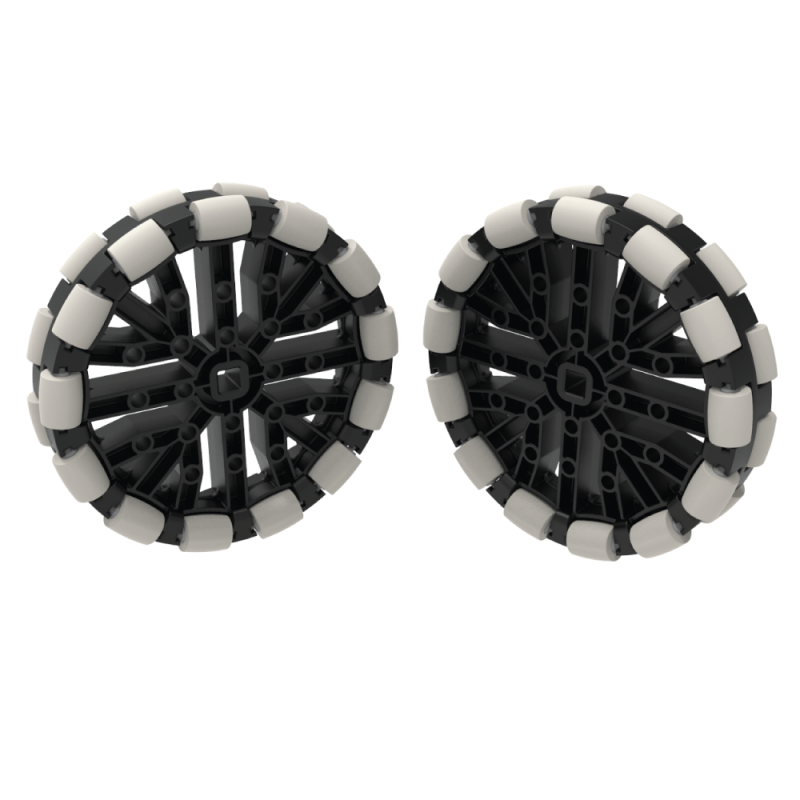
\includegraphics[width=.8\linewidth]{images/Omni Wheels.jpg}
        \caption{Omni-Directional Wheels}
        \label{fig:omni-directional-wheels}
    \end{minipage}%
    \begin{minipage}{.5\textwidth}
        \centering
        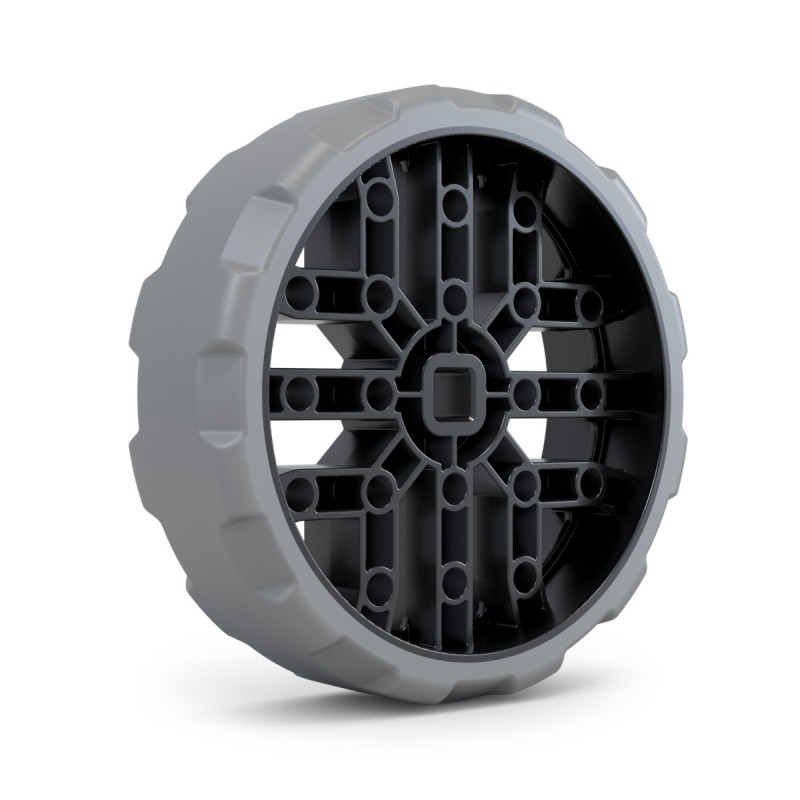
\includegraphics[width=.8\linewidth]{images/Traction Wheels.jpg}
        \caption{Traction Wheels}
        \label{fig:traction-wheels}
    \end{minipage}
    \begin{minipage}{.5\textwidth}
        \centering
        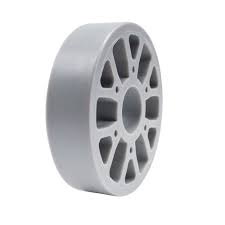
\includegraphics[width=.8\linewidth]{images/Flex Wheels.jpg}
        \caption{Flex Wheels}
        \label{fig:flex-wheels}
    \end{minipage}%
\end{figure}
\pagebreak
\section*{Possible Solution - Cartridge Type}
\noindent 
\textbf{Red Cartridge}

- Spins up to 100 RPM

- Usually used for mechanisms requiring extra torque -- traditionally not a good choice for a drivetrain

\noindent
\textbf{Pros}:
\begin{itemize}
    \item Very strong
    \item Great Acceleration
\end{itemize}
\textbf{Cons}:
\begin{itemize}
    \item Very slow 
    \item Loses torque due to increased friction in the cartridge (36:1 planetary ratio)
\end{itemize}

\noindent 
\textbf{Green Cartridge}

- Spins up to 200 RPM

- Usually used for mechanisms that require a balance between strength and speed -- common because of a shared ratio between 5.5 watt motor

\noindent
\textbf{Pros}:
\begin{itemize}
    \item Has a good balance between speed and torque 
    \item Versitile, easy to gear speed; compatable with 5.5 watt motors
\end{itemize}
\textbf{Cons}:
\begin{itemize}
    \item Often too slow for most drivetrains and lacking enough torque for most mechanisms
\end{itemize}

\textbf{Blue Cartridges}

- Spins up to 600 RPM

- Usually used for mechanisms requiring extra speed such as flywheels

\noindent
\textbf{Pros}:
\begin{itemize}
    \item Very Fast
    \item Causes minimal friction due to the 6:1 planetary ratio
\end{itemize}
\textbf{Cons}:
\begin{itemize}
    \item Significantly lacks torque
\end{itemize}

\begin{figure}[hbt] % Use [hbt!] to place the figures on the same page
    \begin{minipage}{.5\textwidth}
        \centering
        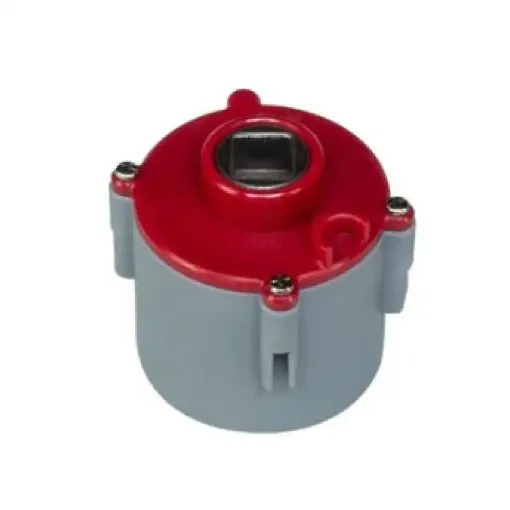
\includegraphics[width=.8\linewidth]{images/Red-Cartridge.png}
        \caption{Red Cartridge}
        \label{fig:red-cartridge}
    \end{minipage}%
    \begin{minipage}{.5\textwidth}
        \centering
        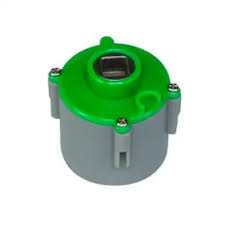
\includegraphics[width=.8\linewidth]{images/Green Cartridge.jpg}
        \caption{Green Cartridge}
        \label{fig:green-cartridge}
    \end{minipage}
    \begin{minipage}{.5\textwidth}
        \centering
        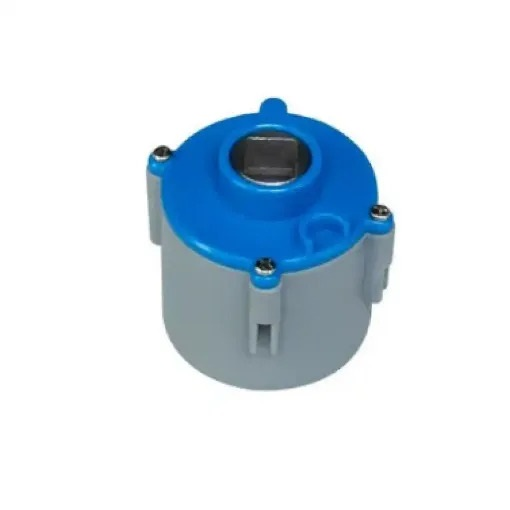
\includegraphics[width=.8\linewidth]{images/Blue-Cartridge.jpg}
        \caption{Blue Cartridge}
        \label{fig:blue-cartridge}
    \end{minipage}%
\end{figure}

% Add in the picture of the motor curve chart here %

% https://kb.vex.com/hc/en-us/articles/360044325872-Understanding-V5-Smart-Motor-11W-Performance %

\pagebreak
\section*{Possible Solution - Drive Type}

\blueref{fig:standard-omnidirectional-wheels}{\textbf{Standard Omnidirectional Wheels -}} 

- Omnidirectional Wheels set up in a tank drive orientation 

- Most common drivetrain type

\noindent
\textbf{Pros}:
\begin{itemize}
    \item Fast
    \item Simple
    \item Compact 
\end{itemize}
\textbf{Cons}:
\begin{itemize}
    \item Roller mechanisms greatly reduce traction due to material type
    \item Moves in only two directions 
\end{itemize}

\blueref{fig:mecanum}{Mecanum Wheels} 

- Specialized wheel design to allow movement in all directions

- Mecanum Wheels set up in a tank drive orientation 

- Second most popular drive design 
\noindent
\textbf{Pros}:
\begin{itemize}
    \item Moves in all directions
    \item Has the power of all motors in all directions
\end{itemize}
\textbf{Cons}:
\begin{itemize}

    \item Bulky
    \item Can be difficult to code
\end{itemize}

\blueref{fig:hexagonal}{\textbf{Holonomic / X-Drive -}} 

- Omnidirectional Wheels set up in a hexagonal orientation

- Two sets of parallel lines with each wheel oriented 45 degrees from a standard tanks drive 

- Third most common drive-train type 

\noindent
\textbf{Pros}:
\begin{itemize}
    \item Moves in all directions
    \item Less bulky than Mecanum drive 
    \item Has the power of all motors in all directions
\end{itemize}
\textbf{Cons}:
\begin{itemize}
    \item Complex Programming 
    \item Still comparatively large 
    \item Half as fast in all directions
\end{itemize}

\blueref{fig:h-drive}{\textbf{H-Drive -}} 

- Five omnidirectional wheels set up to look like the letter "H"

- Four wheels set up in a tank drive orientation 

- The fifth wheel is perpendicular to the orientation of the others and moves the drive side to side
\noindent
\textbf{Pros}:
\begin{itemize}
    \item Moves in all directions
    \item Simple
    \item Moves fast in all directions
\end{itemize}
\textbf{Cons}:
\begin{itemize}
    \item Complex programming
    \item Only has the power of 1 motor when moving side to side 
    \item Requires all wheels to be omnidirectional
\end{itemize}

\blueref{fig:traction-wheel-drive}{\textbf{All Traction Wheel Drive -}} 

- Wheel design for more traction

- Traction wheels set up in a tank drive orientation 

\noindent
\textbf{Pros}:
\begin{itemize}
    \item  Excellent traction
    \item Simple
    \item Compact 
\end{itemize}
\textbf{Cons}:
\begin{itemize}

    \item Slow turning
\end{itemize}

\blueref{fig:omnidirectional-and-traction-wheels}{\textbf{Omnidirectinal and Traction Wheels -}} 

- Omnidirectional wheels and Traction wheels set up in a tank drive orientation 

- One or two traction wheels in the middle and omni wheels to the front and rear of it 

\noindent
\textbf{Pros}:
\begin{itemize}
    \item Good traction
    \item Simple
    \item Compact 
\end{itemize}
\textbf{Cons}:
\begin{itemize}
    \item Doens't allow for Omnidirectional driving styles
\end{itemize}

\blueref{fig:tank-treads}{\textbf{Tank Tread -}} 

- Sprockets connected by tread in the VEX
tank tread kit

- Sprockets are oriented in a trIangle that is parallel
to the ground

\noindent
\textbf{Pros}:
\begin{itemize}
    \item Great traction
    \item Strong pushing force
    \item Great at climbing over objects 
\end{itemize}
\textbf{Cons}:
\begin{itemize}
    \item Very slow
    \item Very slow turning 
    \item Tracks can fall apart leaving the robot immobile
\end{itemize}

\blueref{fig:walking-robot}{\textbf{Walking Robot -}} 
- C-Channels that move back and forth

- Looks like a person walking

\noindent
\textbf{Pros}:
\begin{itemize} 
    \item Unique 
    \item Moves over rough terrain
\end{itemize}
\textbf{Cons}:
\begin{itemize}
    \item Very tall
    \item Extremely slow
    \item Does not turn
    \item Looks clunky
\end{itemize}
\begin{center}
    \textbf{Hand drawn images of all Drive Types on following page}
\end{center}
\pagebreak
\begin{figure}[hbt!] % Use [hbt!] to place the figures on the same page
    \begin{minipage}{.5\textwidth}
        \centering
        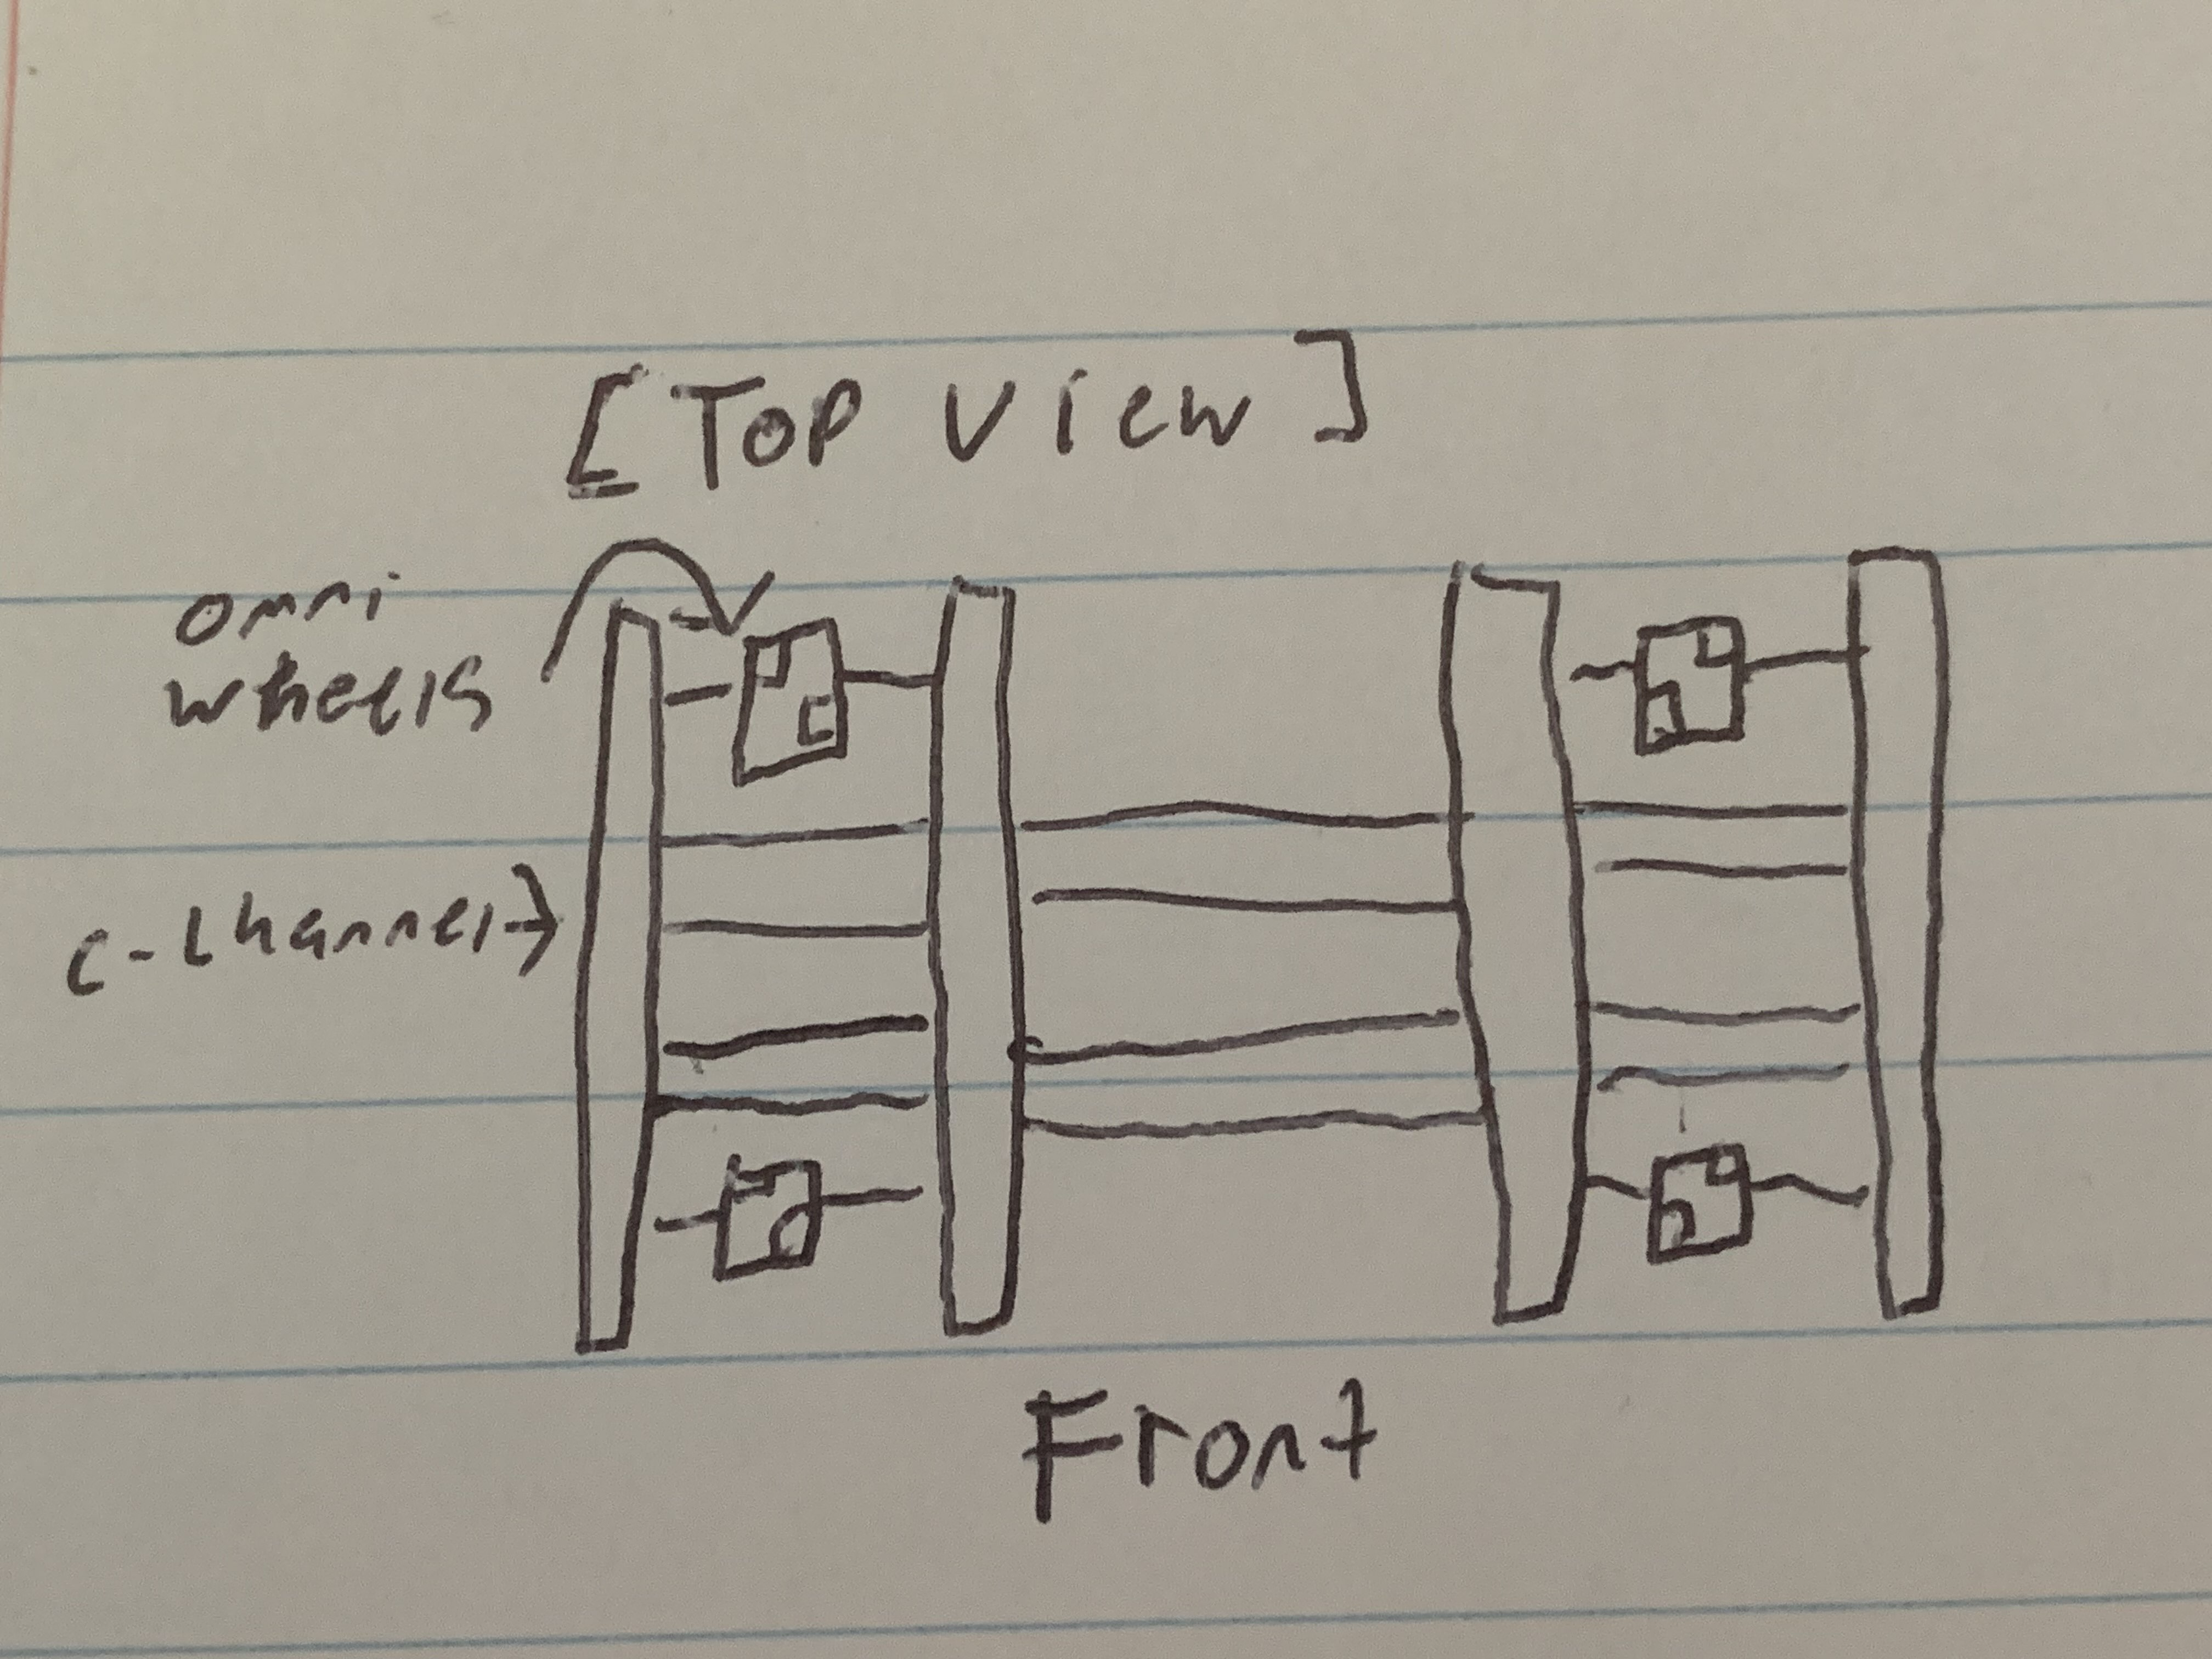
\includegraphics[width=.8\linewidth]{images/Omni Drive.jpg}
        \caption{Standard Omnidirectional} %re draw this with six wheels
        \label{fig:standard-omnidirectional-wheels}
    \end{minipage}%
    \begin{minipage}{.5\textwidth}
        \centering
        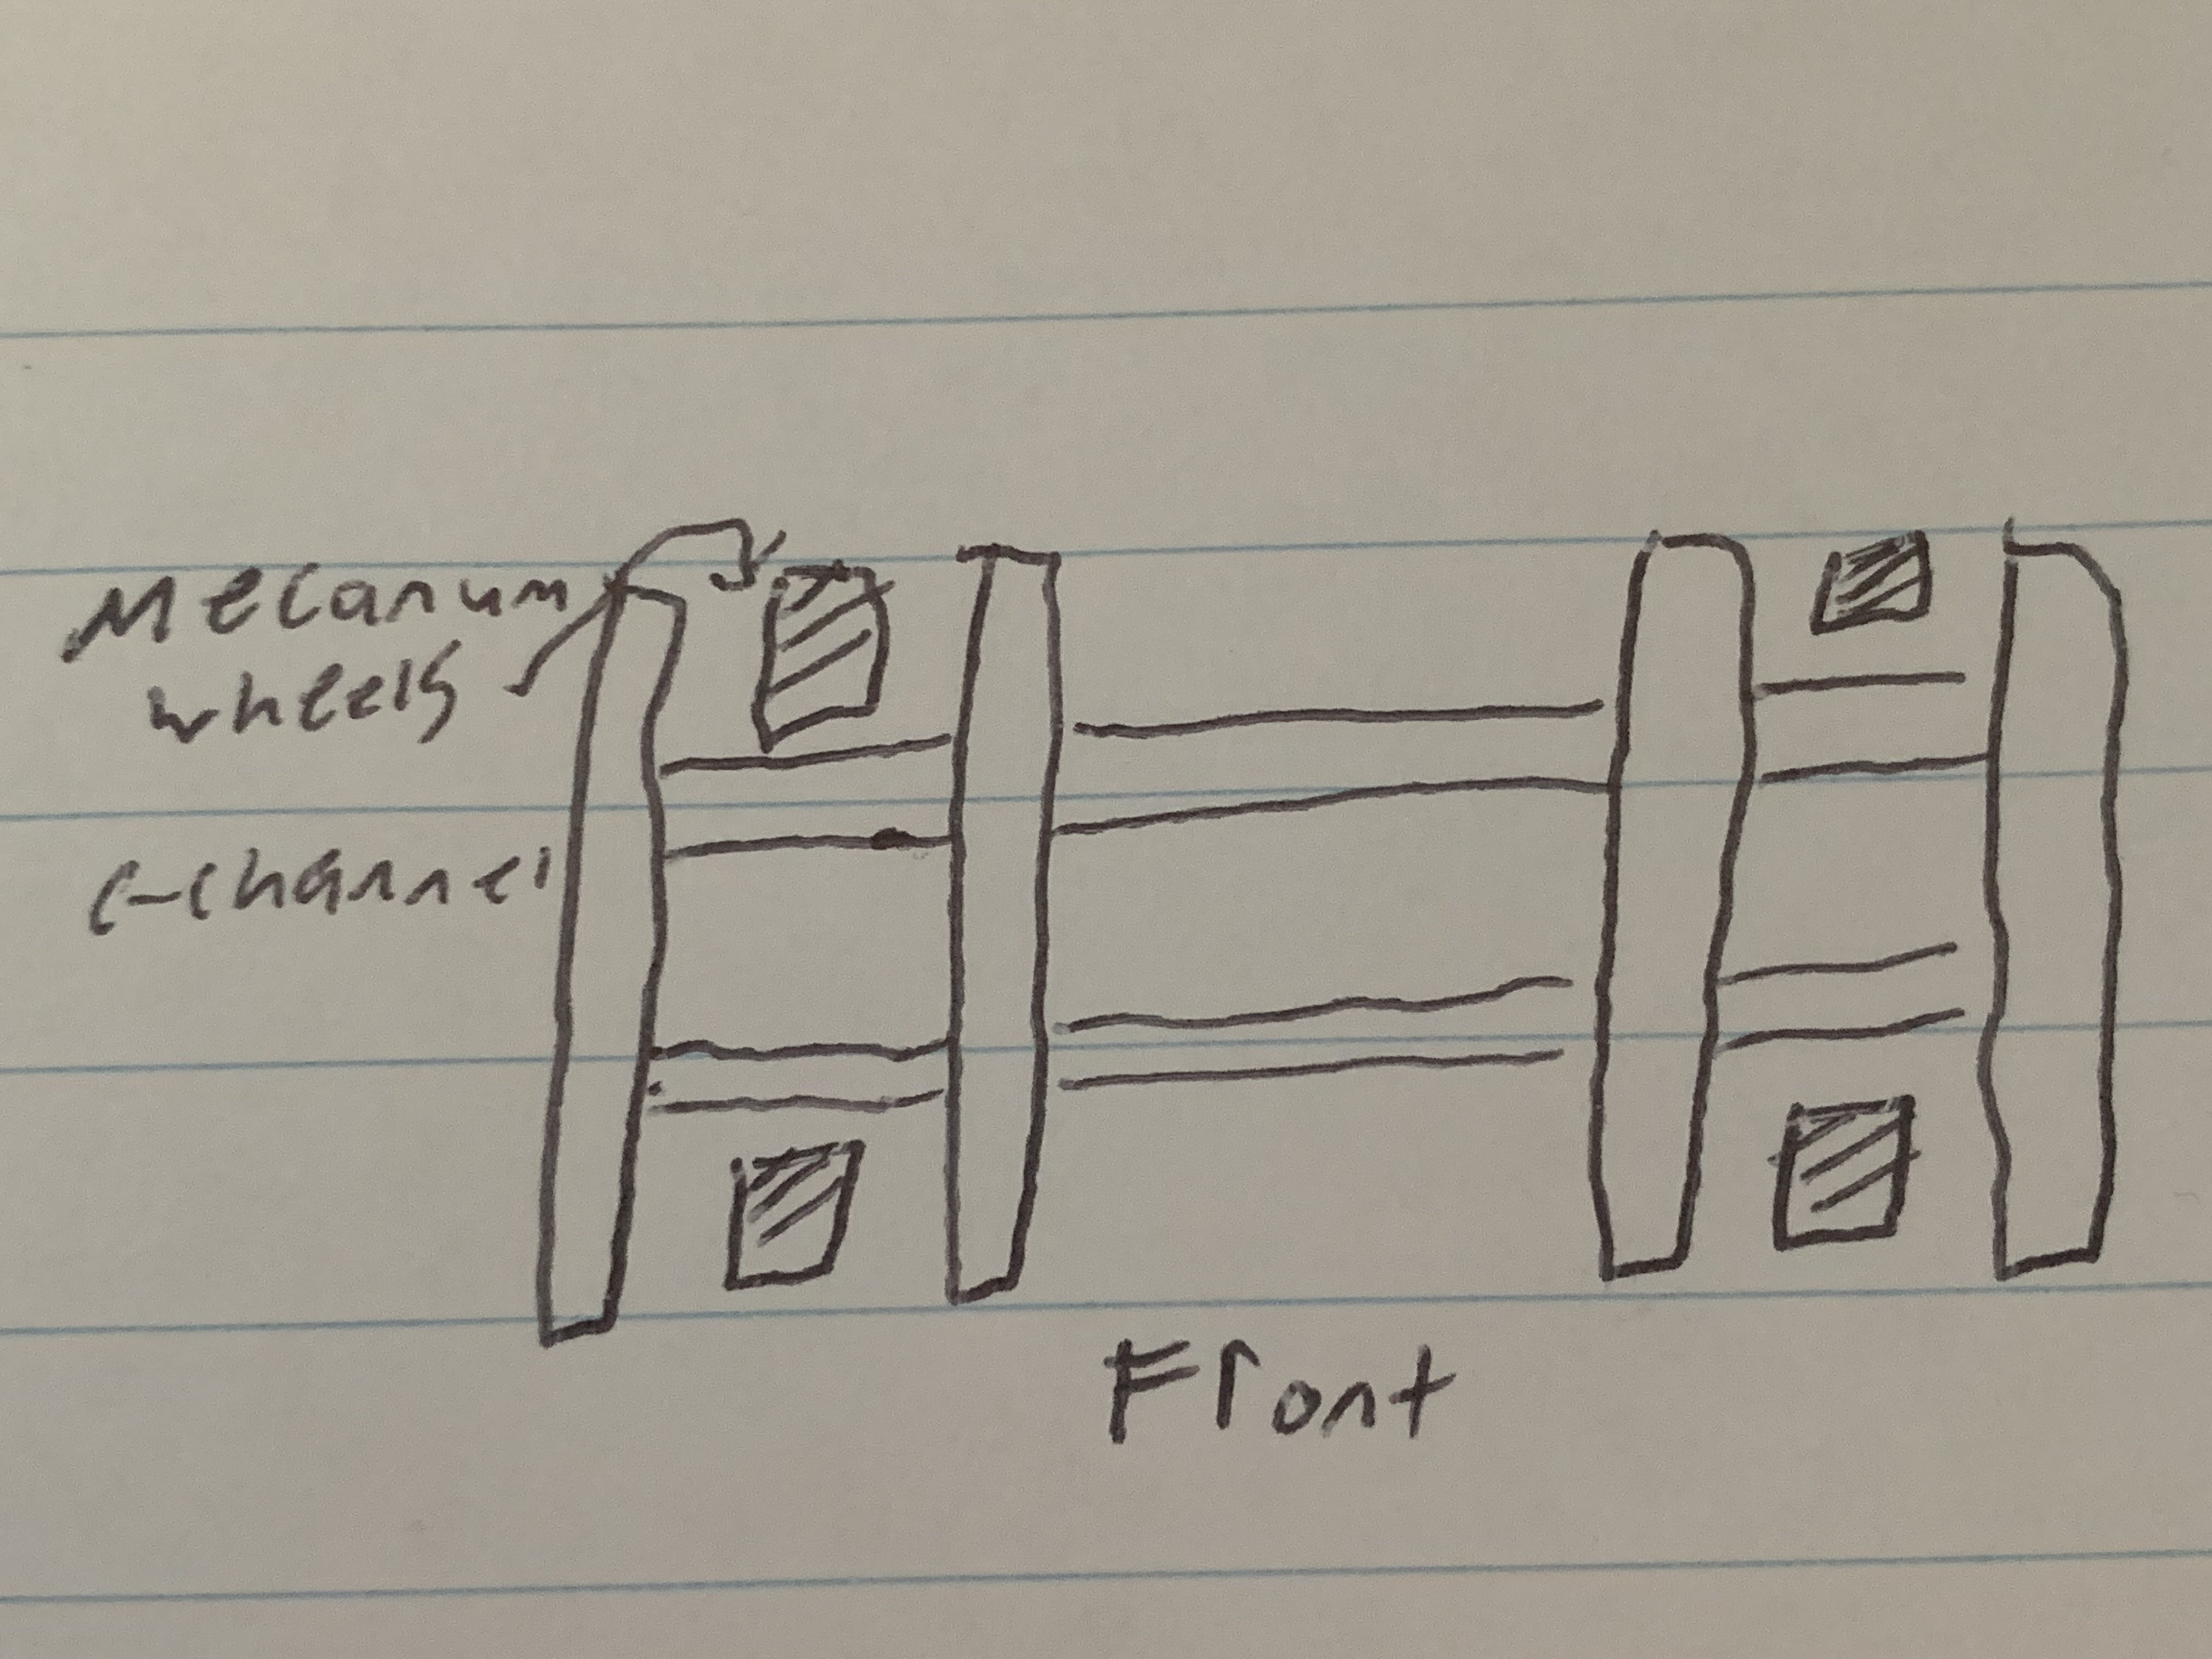
\includegraphics[width=.8\linewidth]{images/Mecanum Drive.jpg}
        \caption{Mecanum}
        \label{fig:mecanum}
    \end{minipage}
    \begin{minipage}{.5\textwidth}
        \centering
        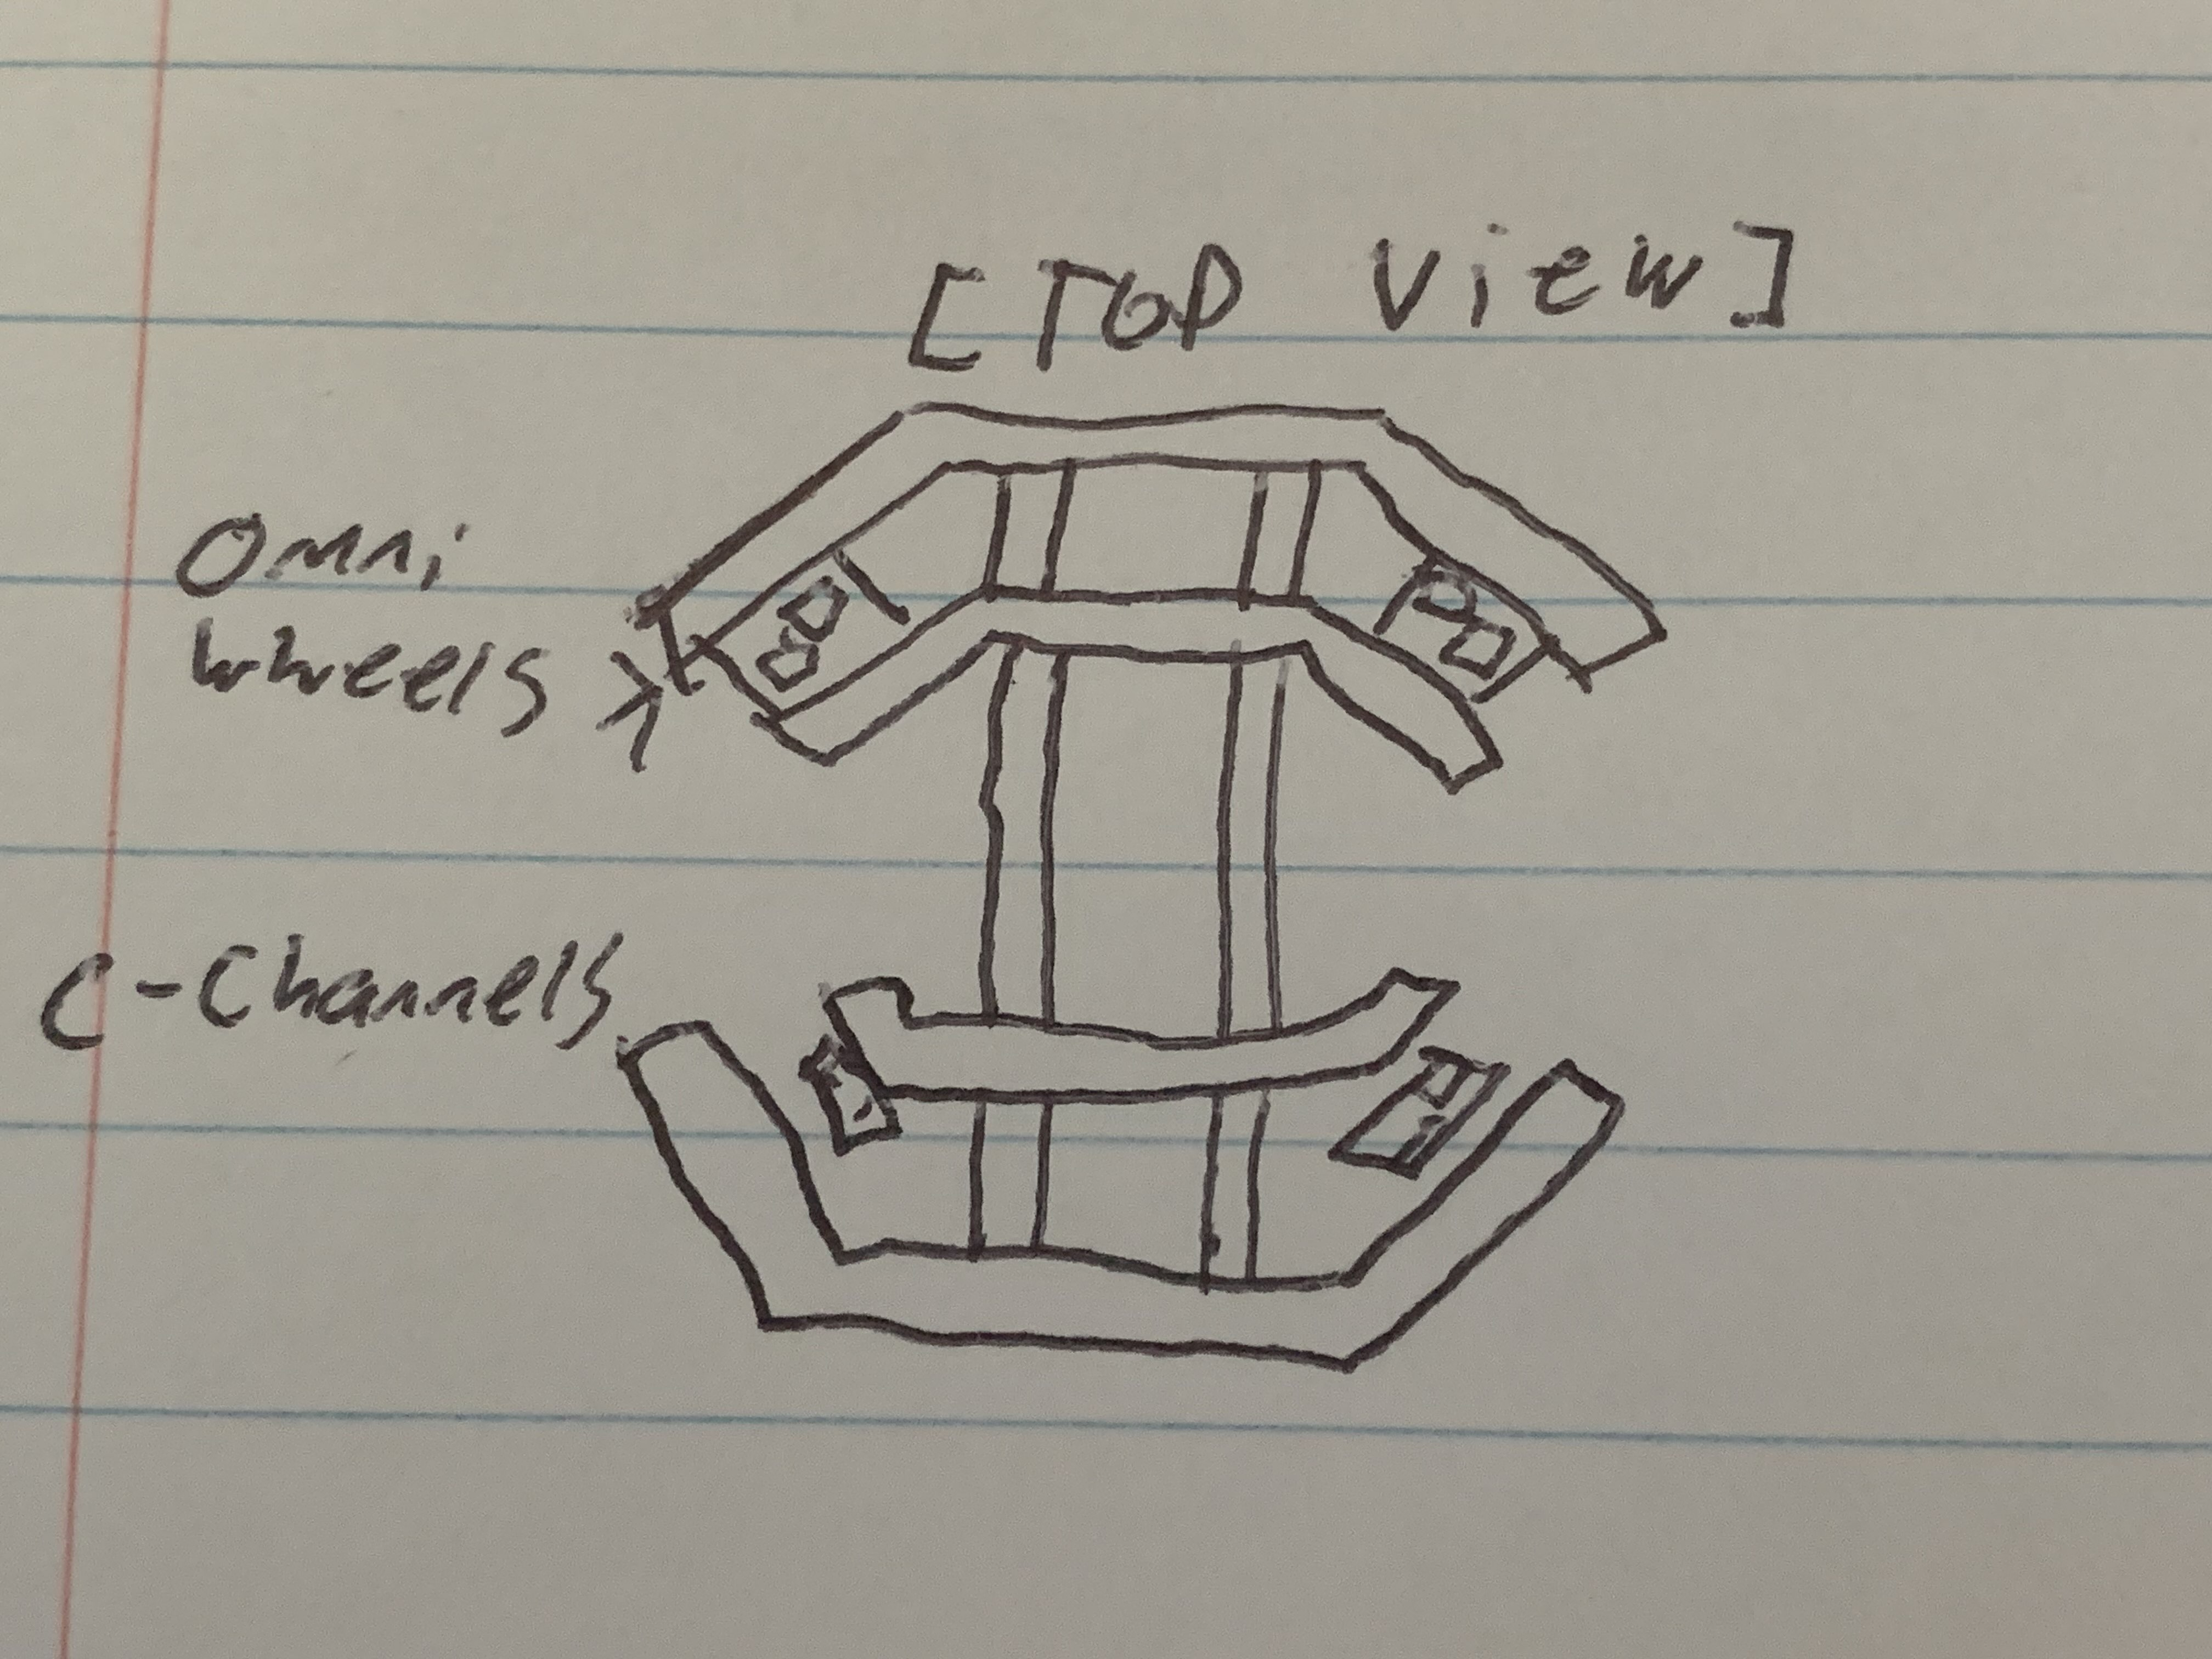
\includegraphics[width=.8\linewidth]{images/Hexagonal Omni Wheels.jpg}
        \caption{Holonomic / X-Drive}
        \label{fig:hexagonal}
    \end{minipage}%
    \begin{minipage}{.5\textwidth}
        \centering
        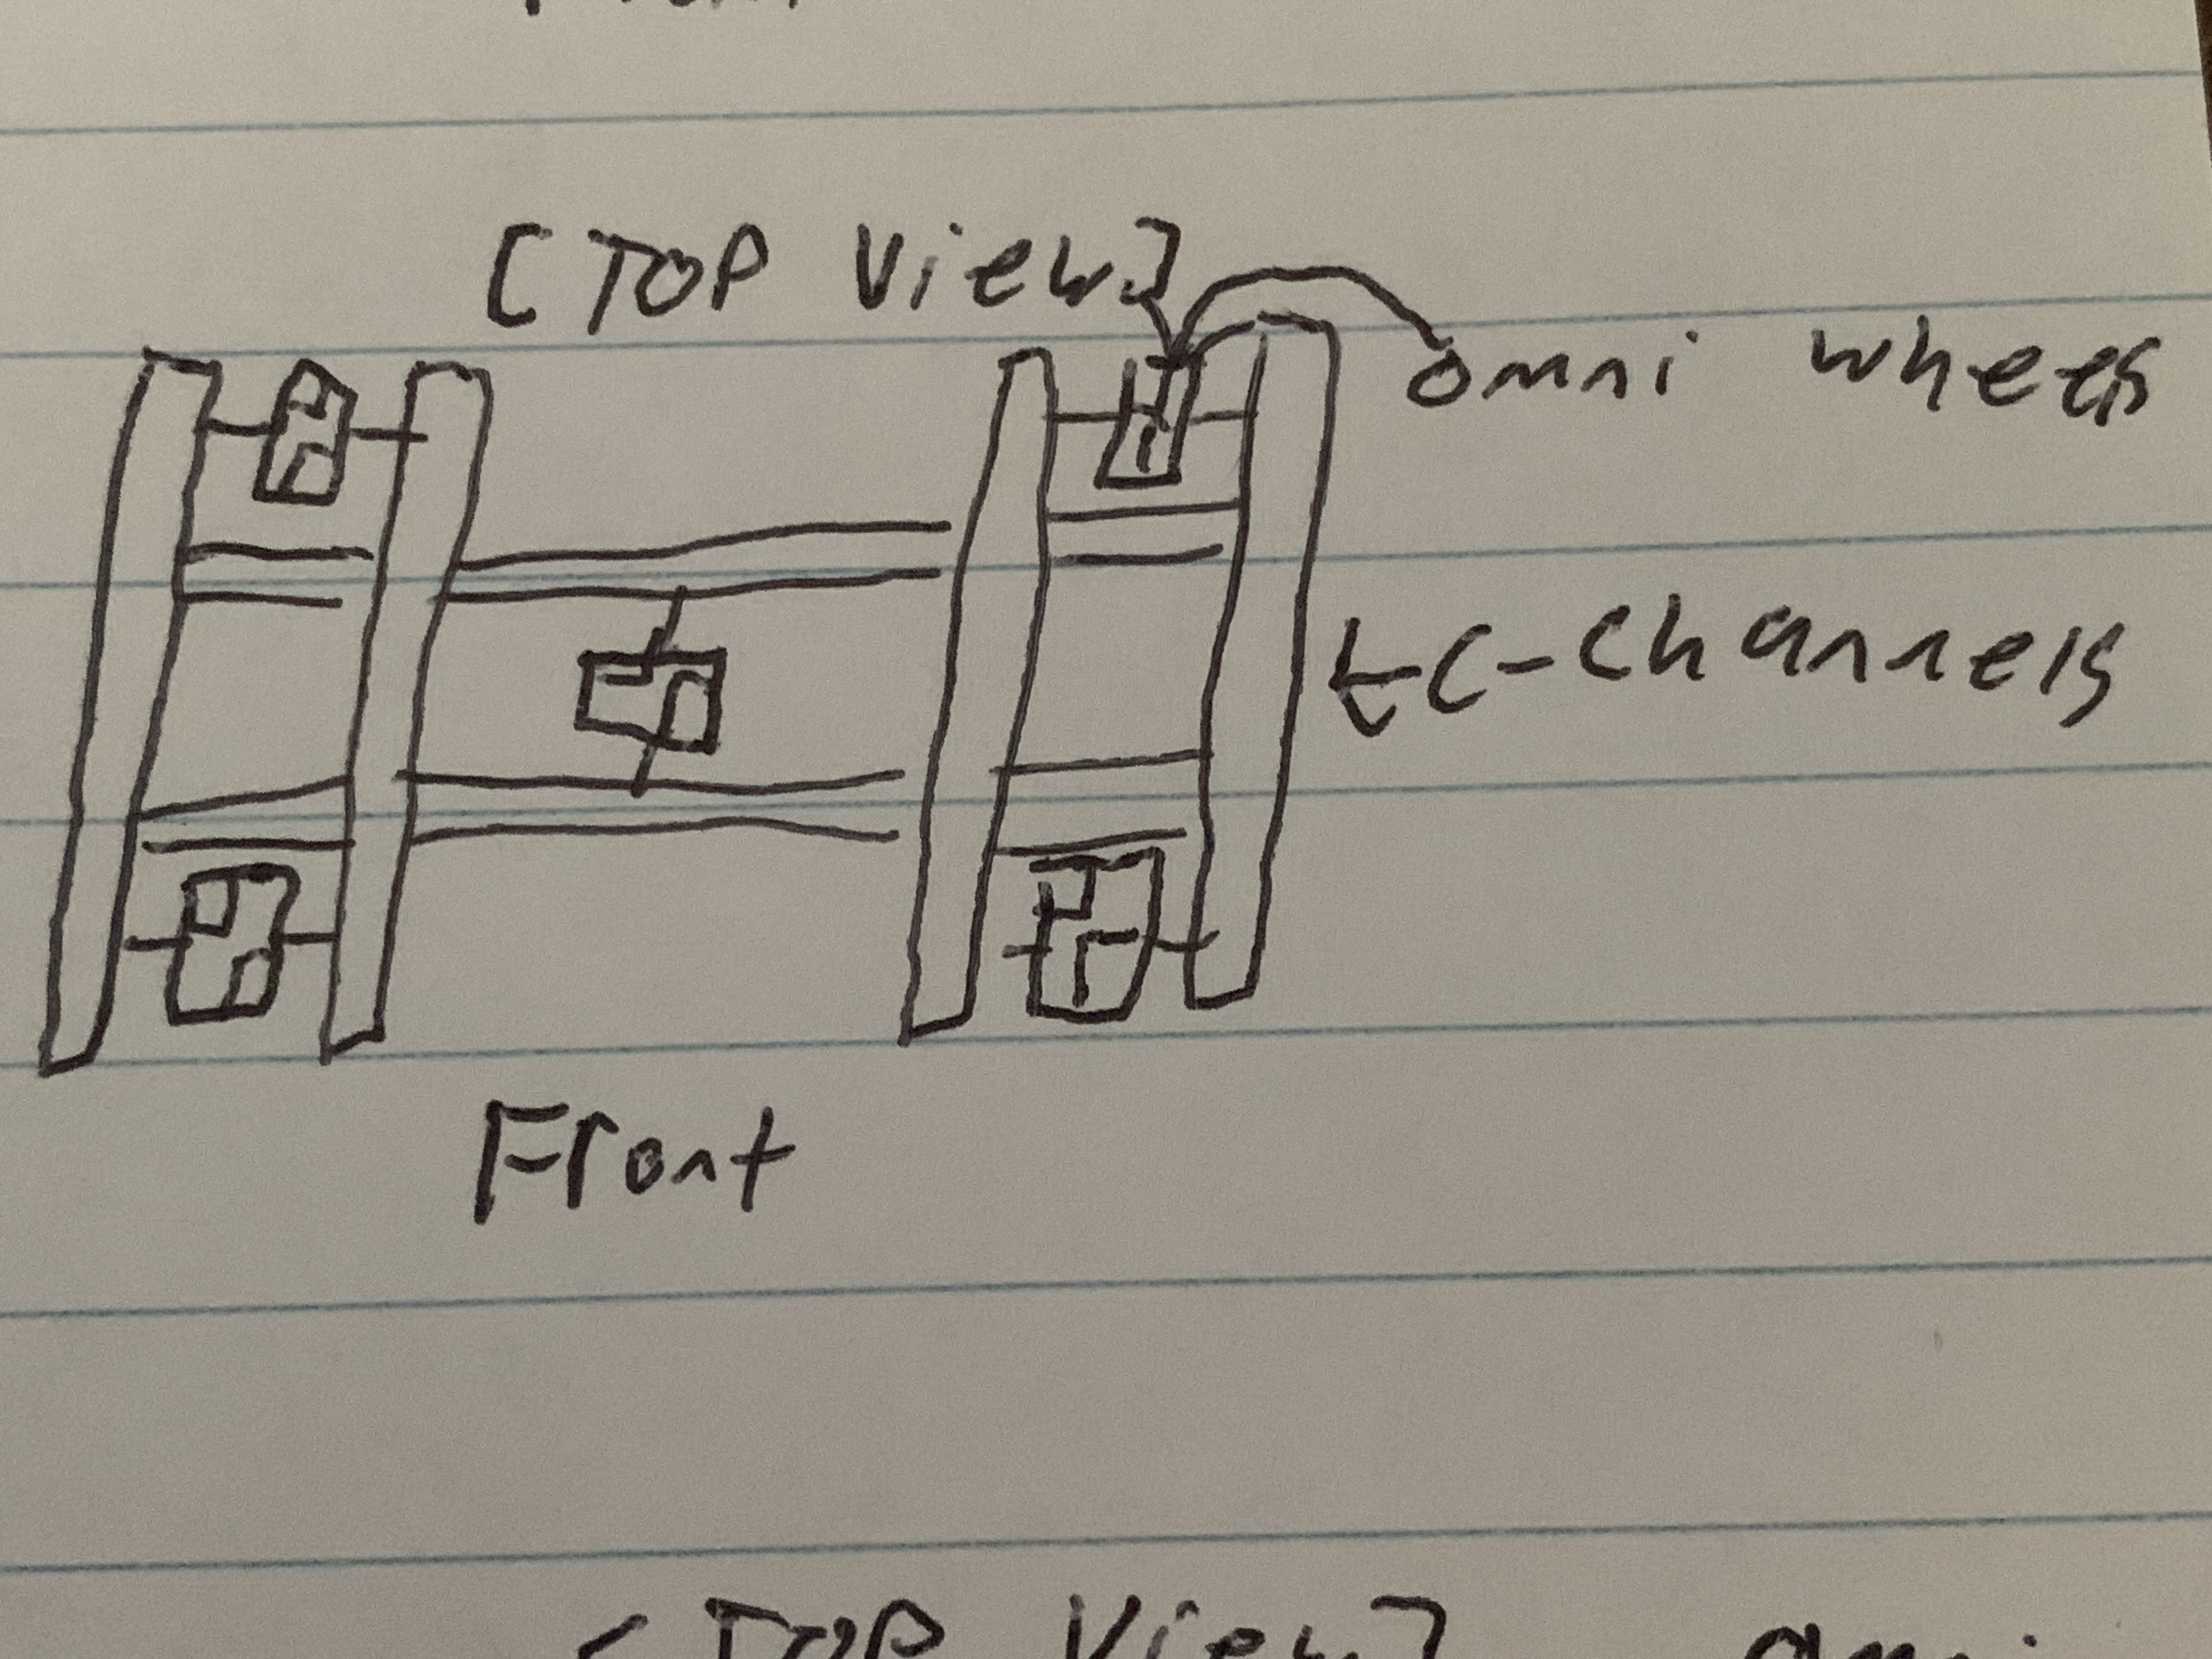
\includegraphics[width=.8\linewidth]{images/5 Omni Wheels.jpg}
        \caption{H-Drive}
        \label{fig:h-drive}
    \end{minipage}
    \begin{minipage}{.5\textwidth}
        \centering
        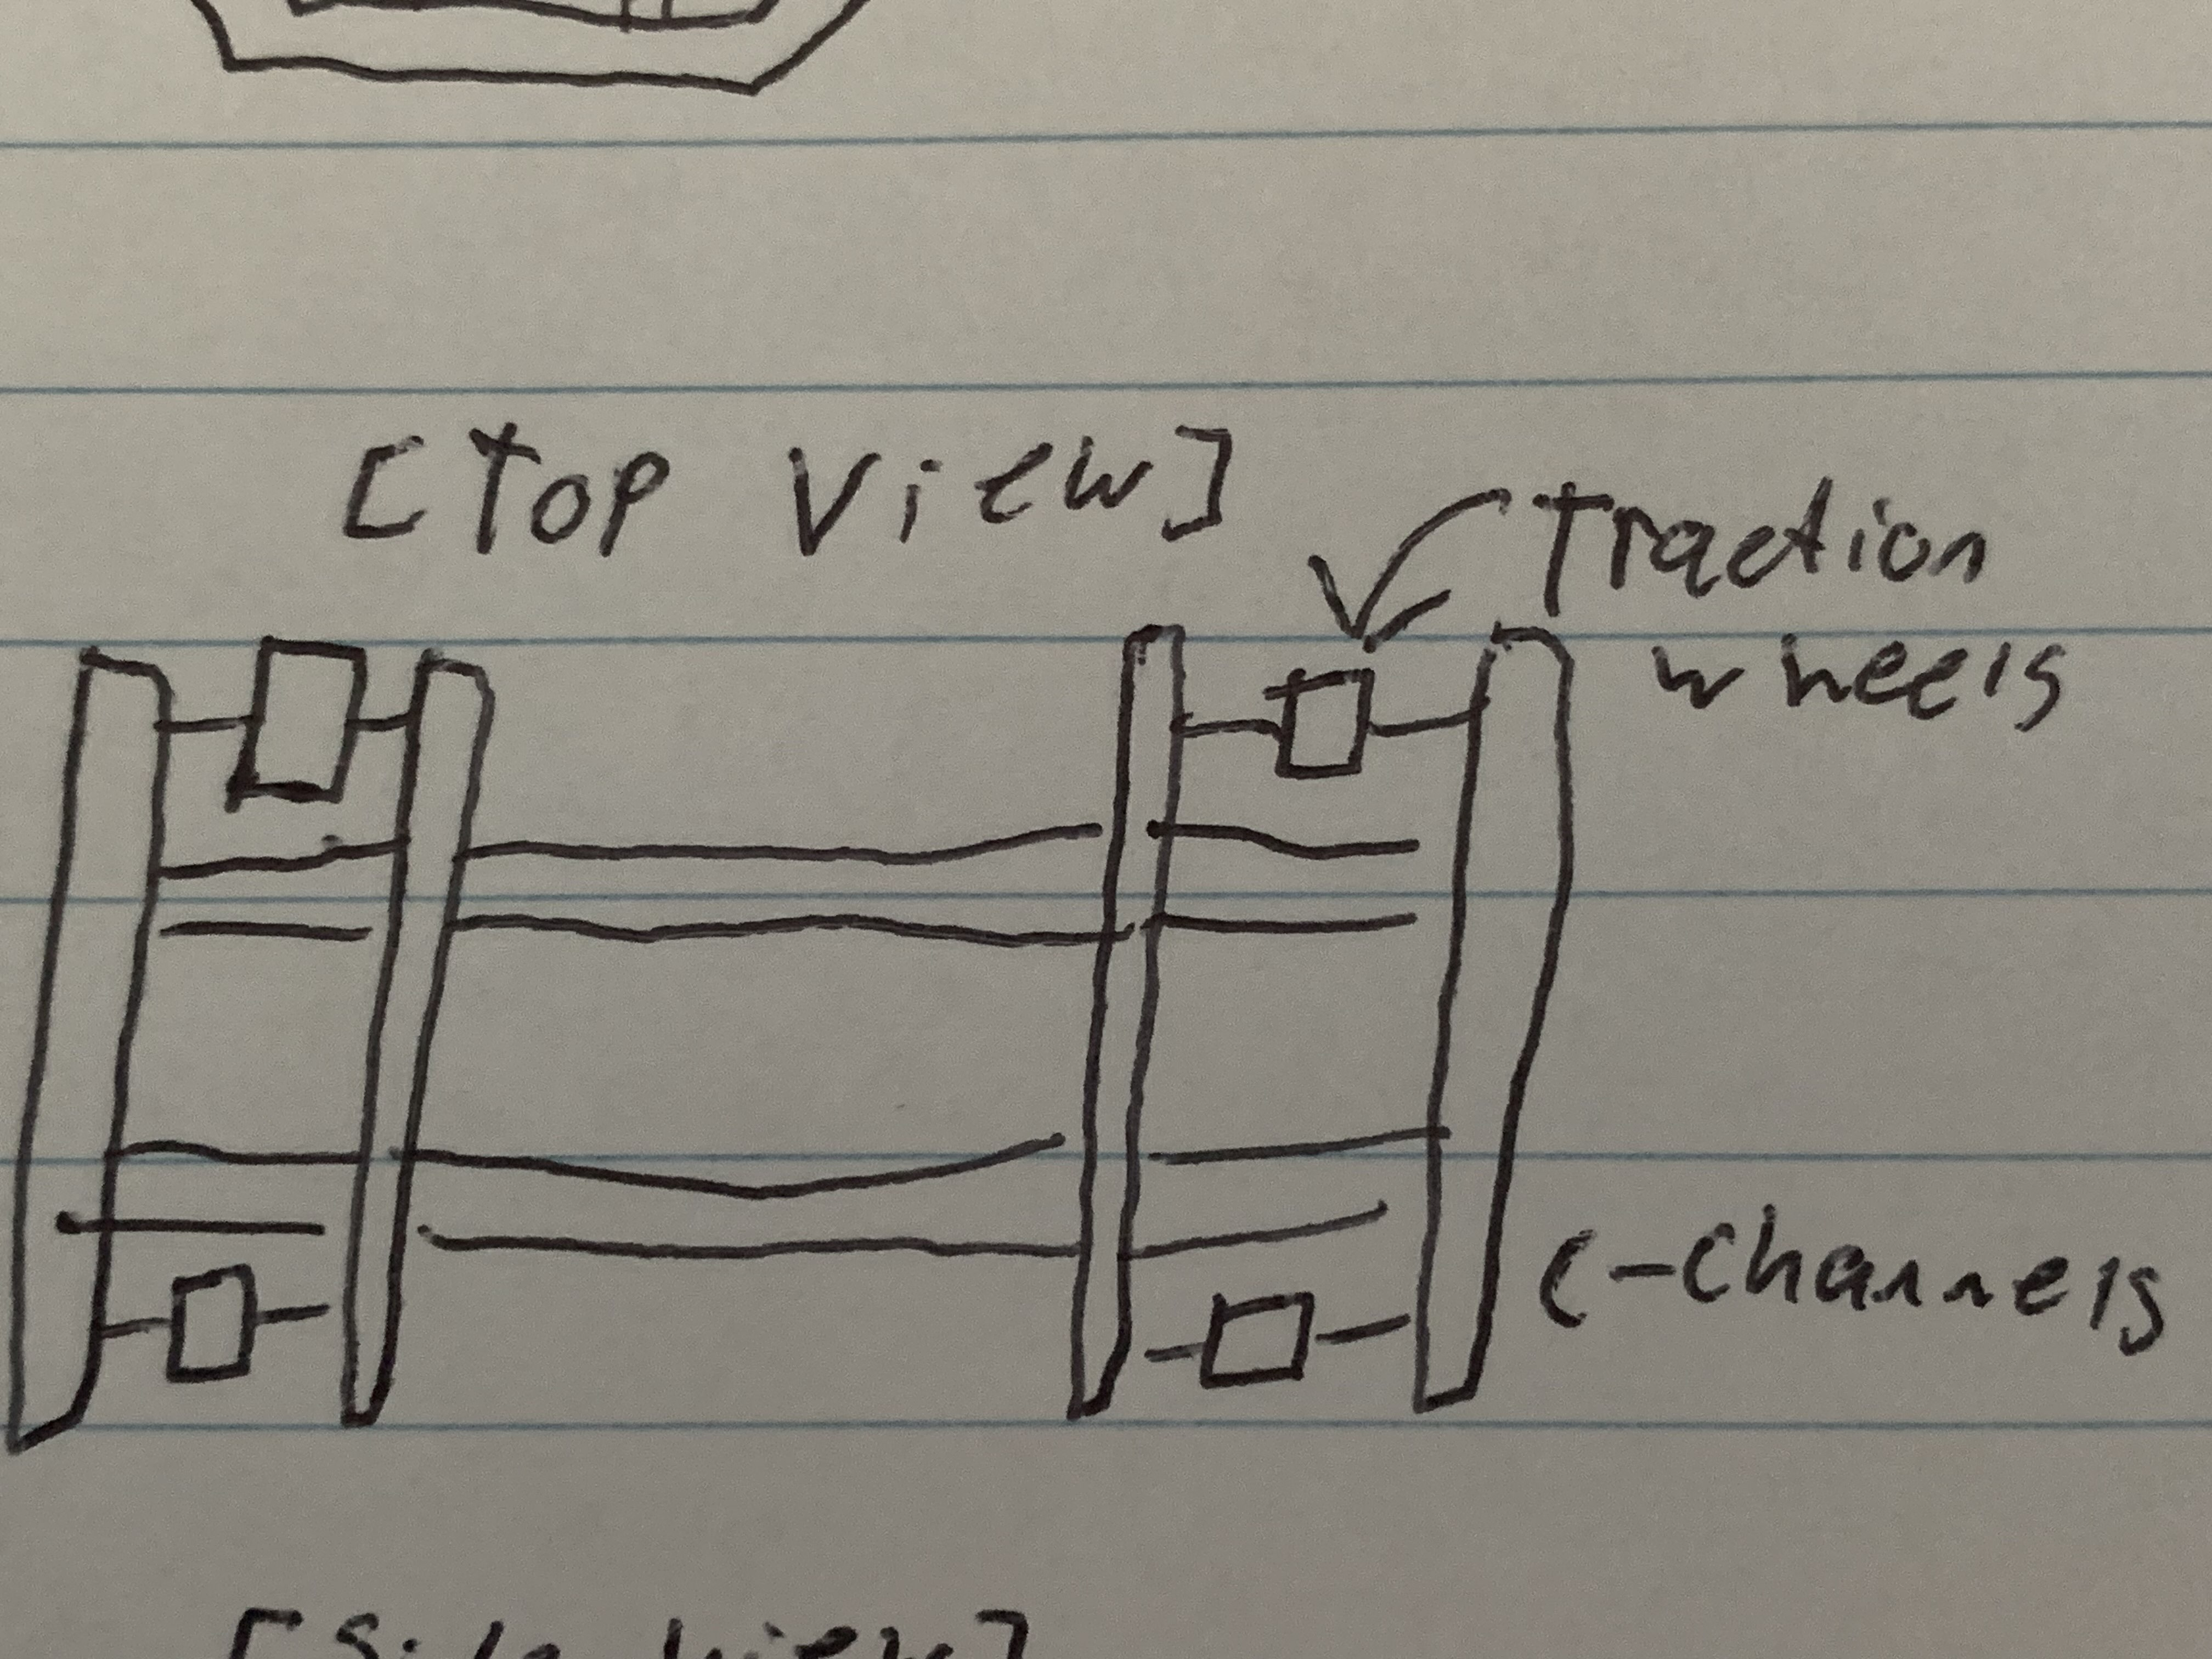
\includegraphics[width=.8\linewidth]{images/Traction Wheel Drive.jpg}
        \caption{Traction Wheel Drive}
        \label{fig:traction-wheel-drive}
    \end{minipage}%
    \begin{minipage}{.5\textwidth}
        \centering
        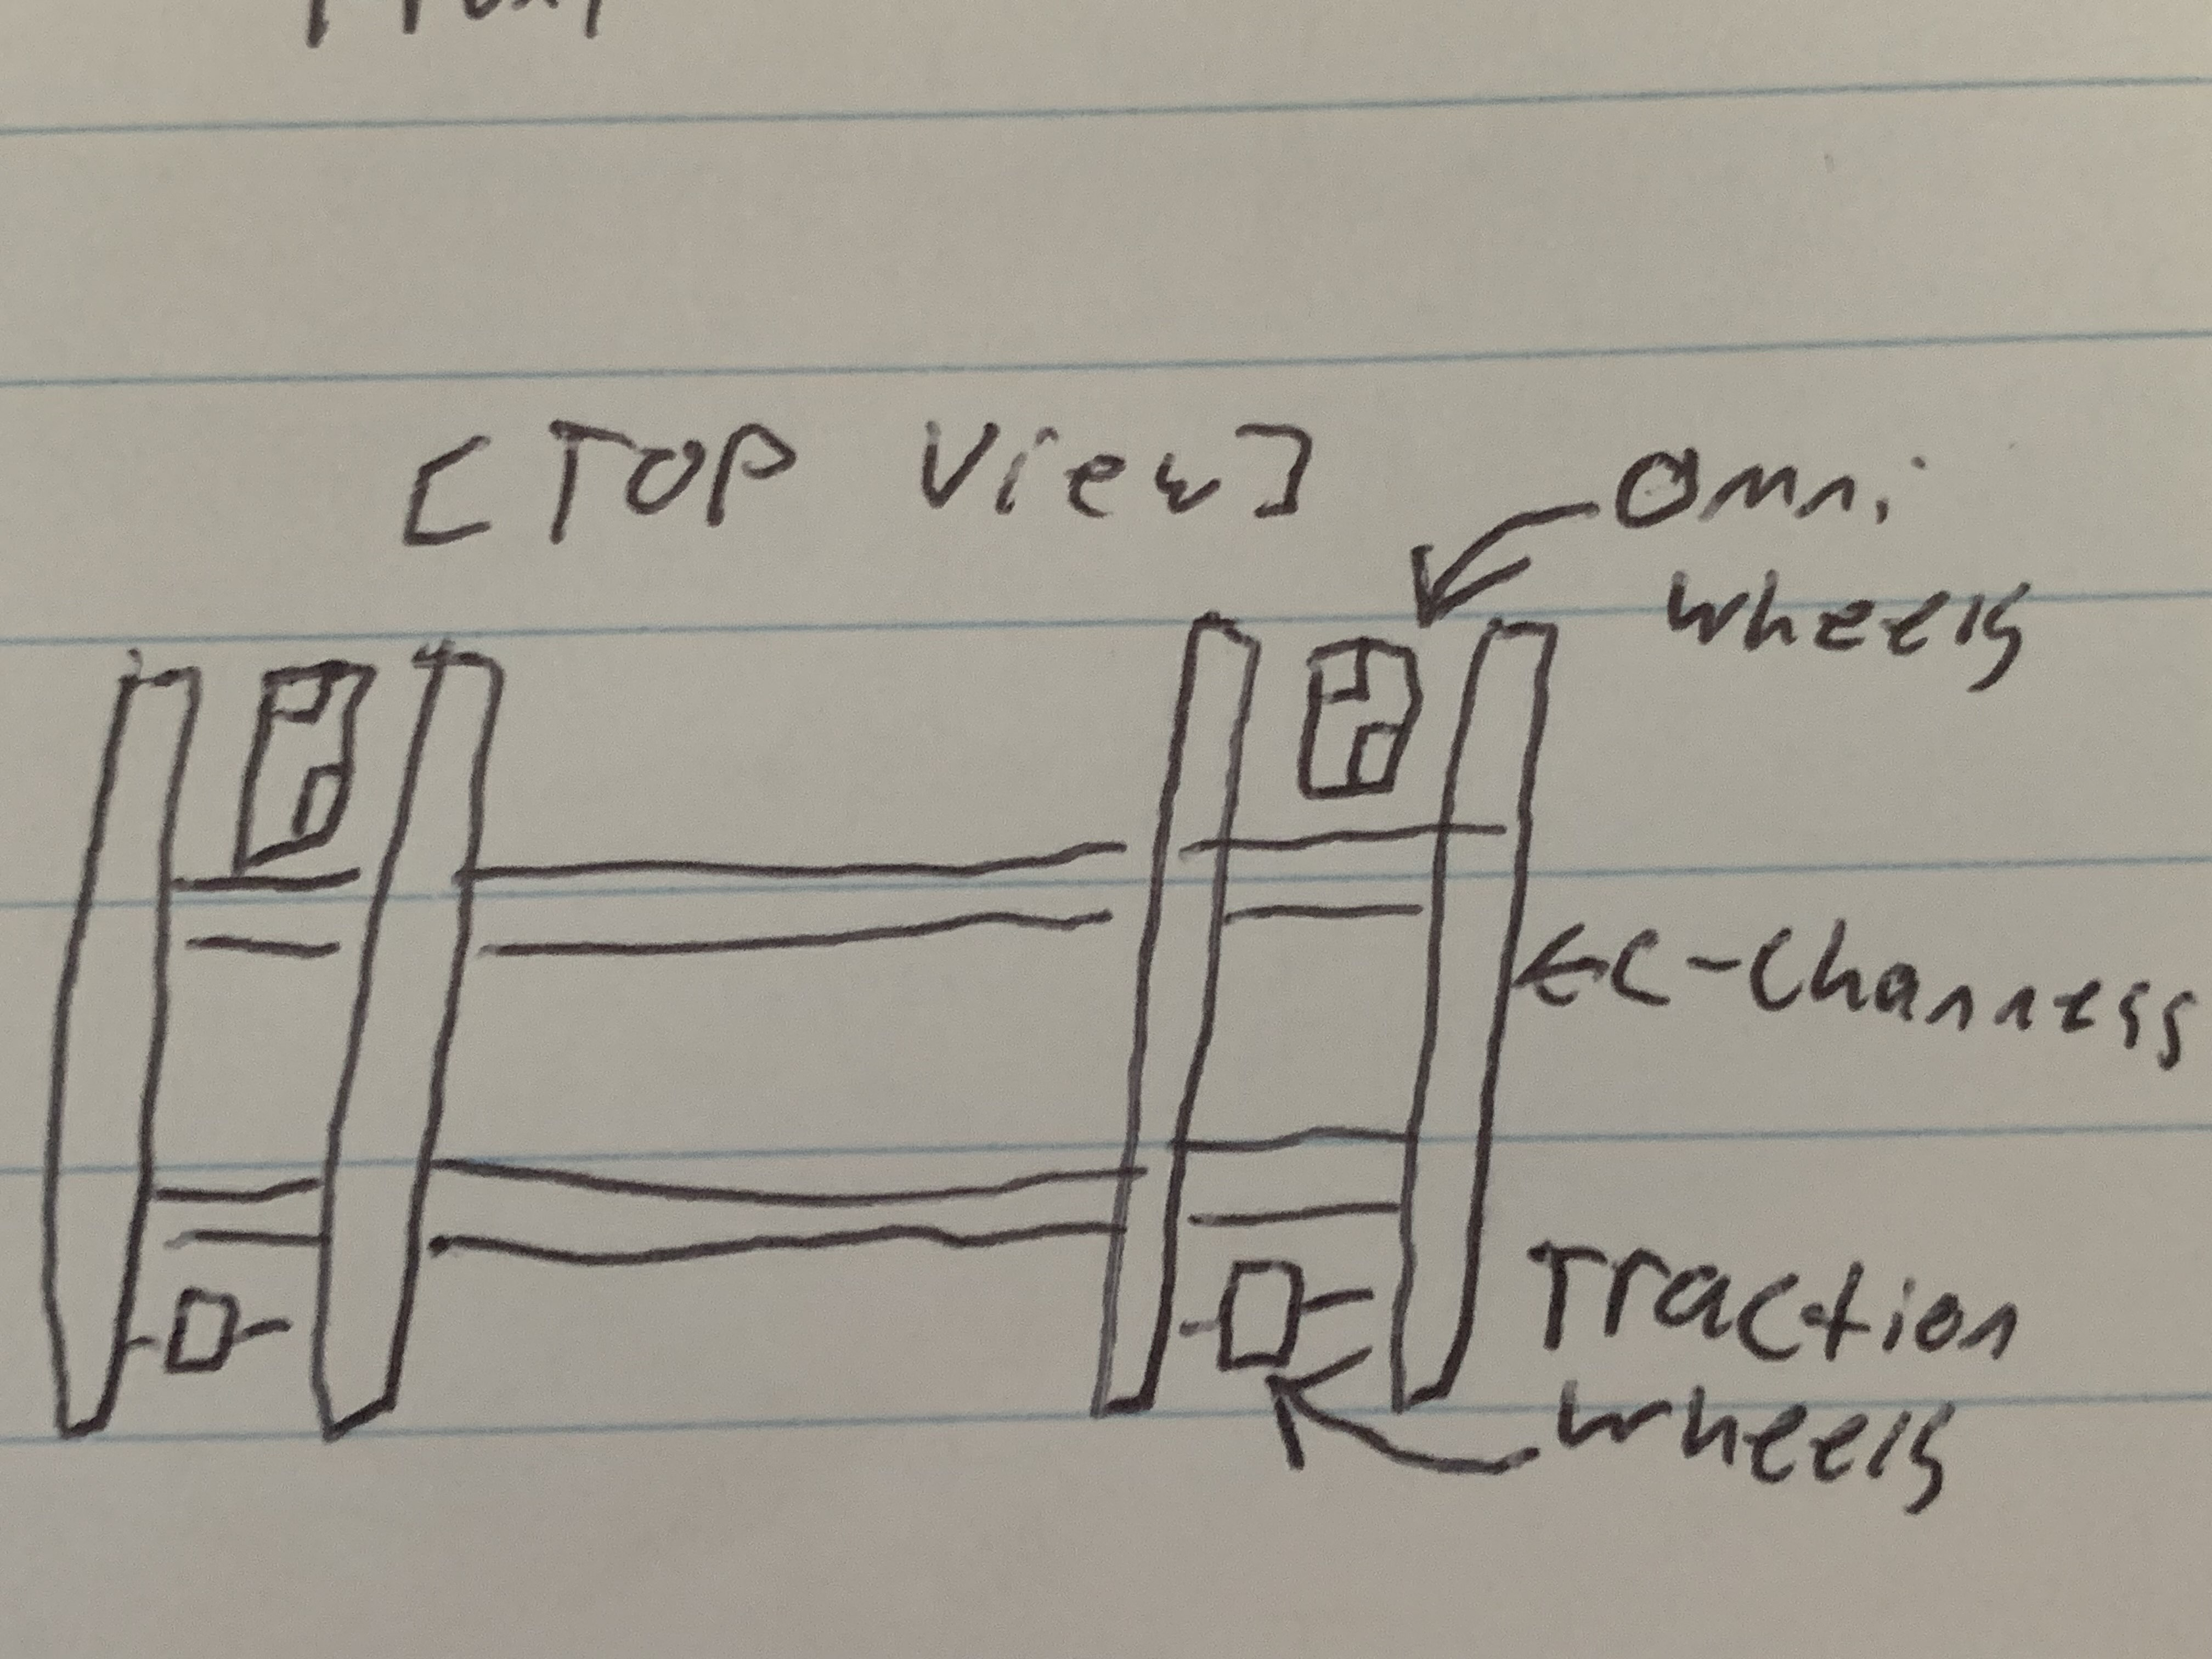
\includegraphics[width=.8\linewidth]{images/Omni and Traction Wheel Drive.jpg}
        \caption{Omnidirectional and Traction Wheels} %redraw this to look like our drive setup, traction in the middle and omnis on the outside
        %on it
        \label{fig:omnidirectional-and-traction-wheels}
    \end{minipage}
     \begin{minipage}{.5\textwidth}
        \centering
        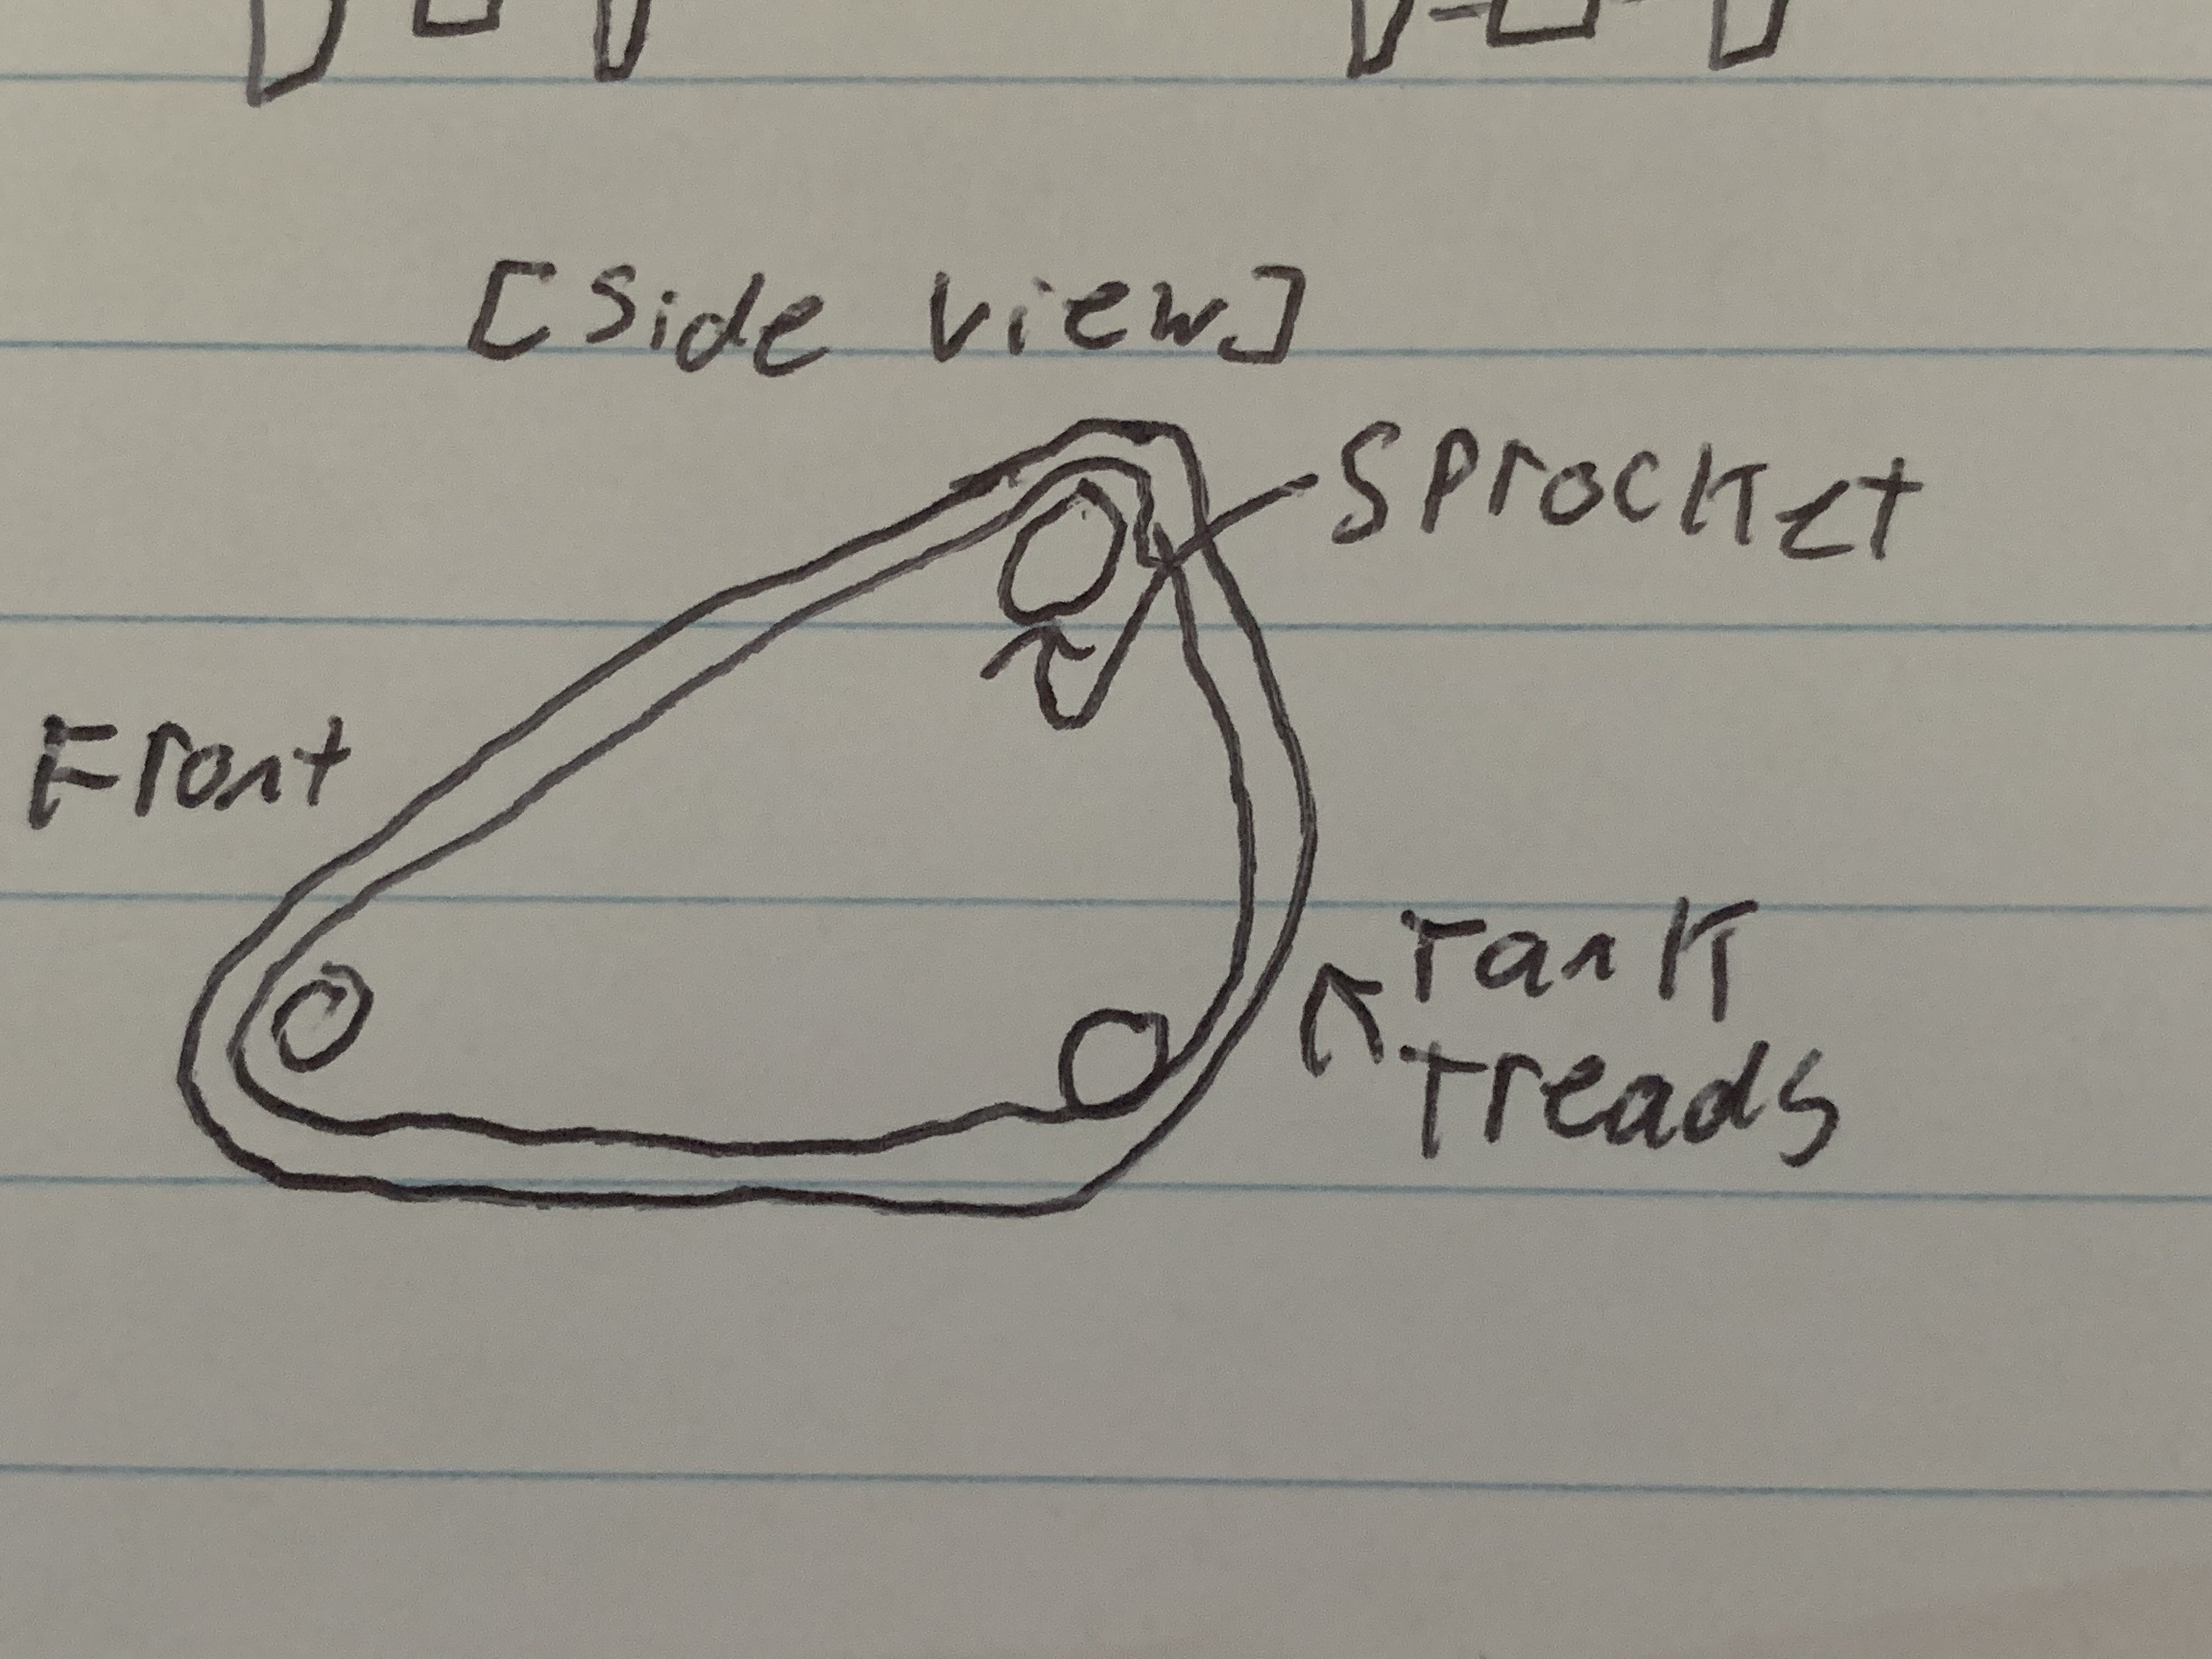
\includegraphics[width=.8\linewidth]{images/Tank - Treads.jpg}
        \caption{Tank Treads}
        \label{fig:tank-treads}
    \end{minipage}
     \begin{minipage}{.5\textwidth}
        \centering
        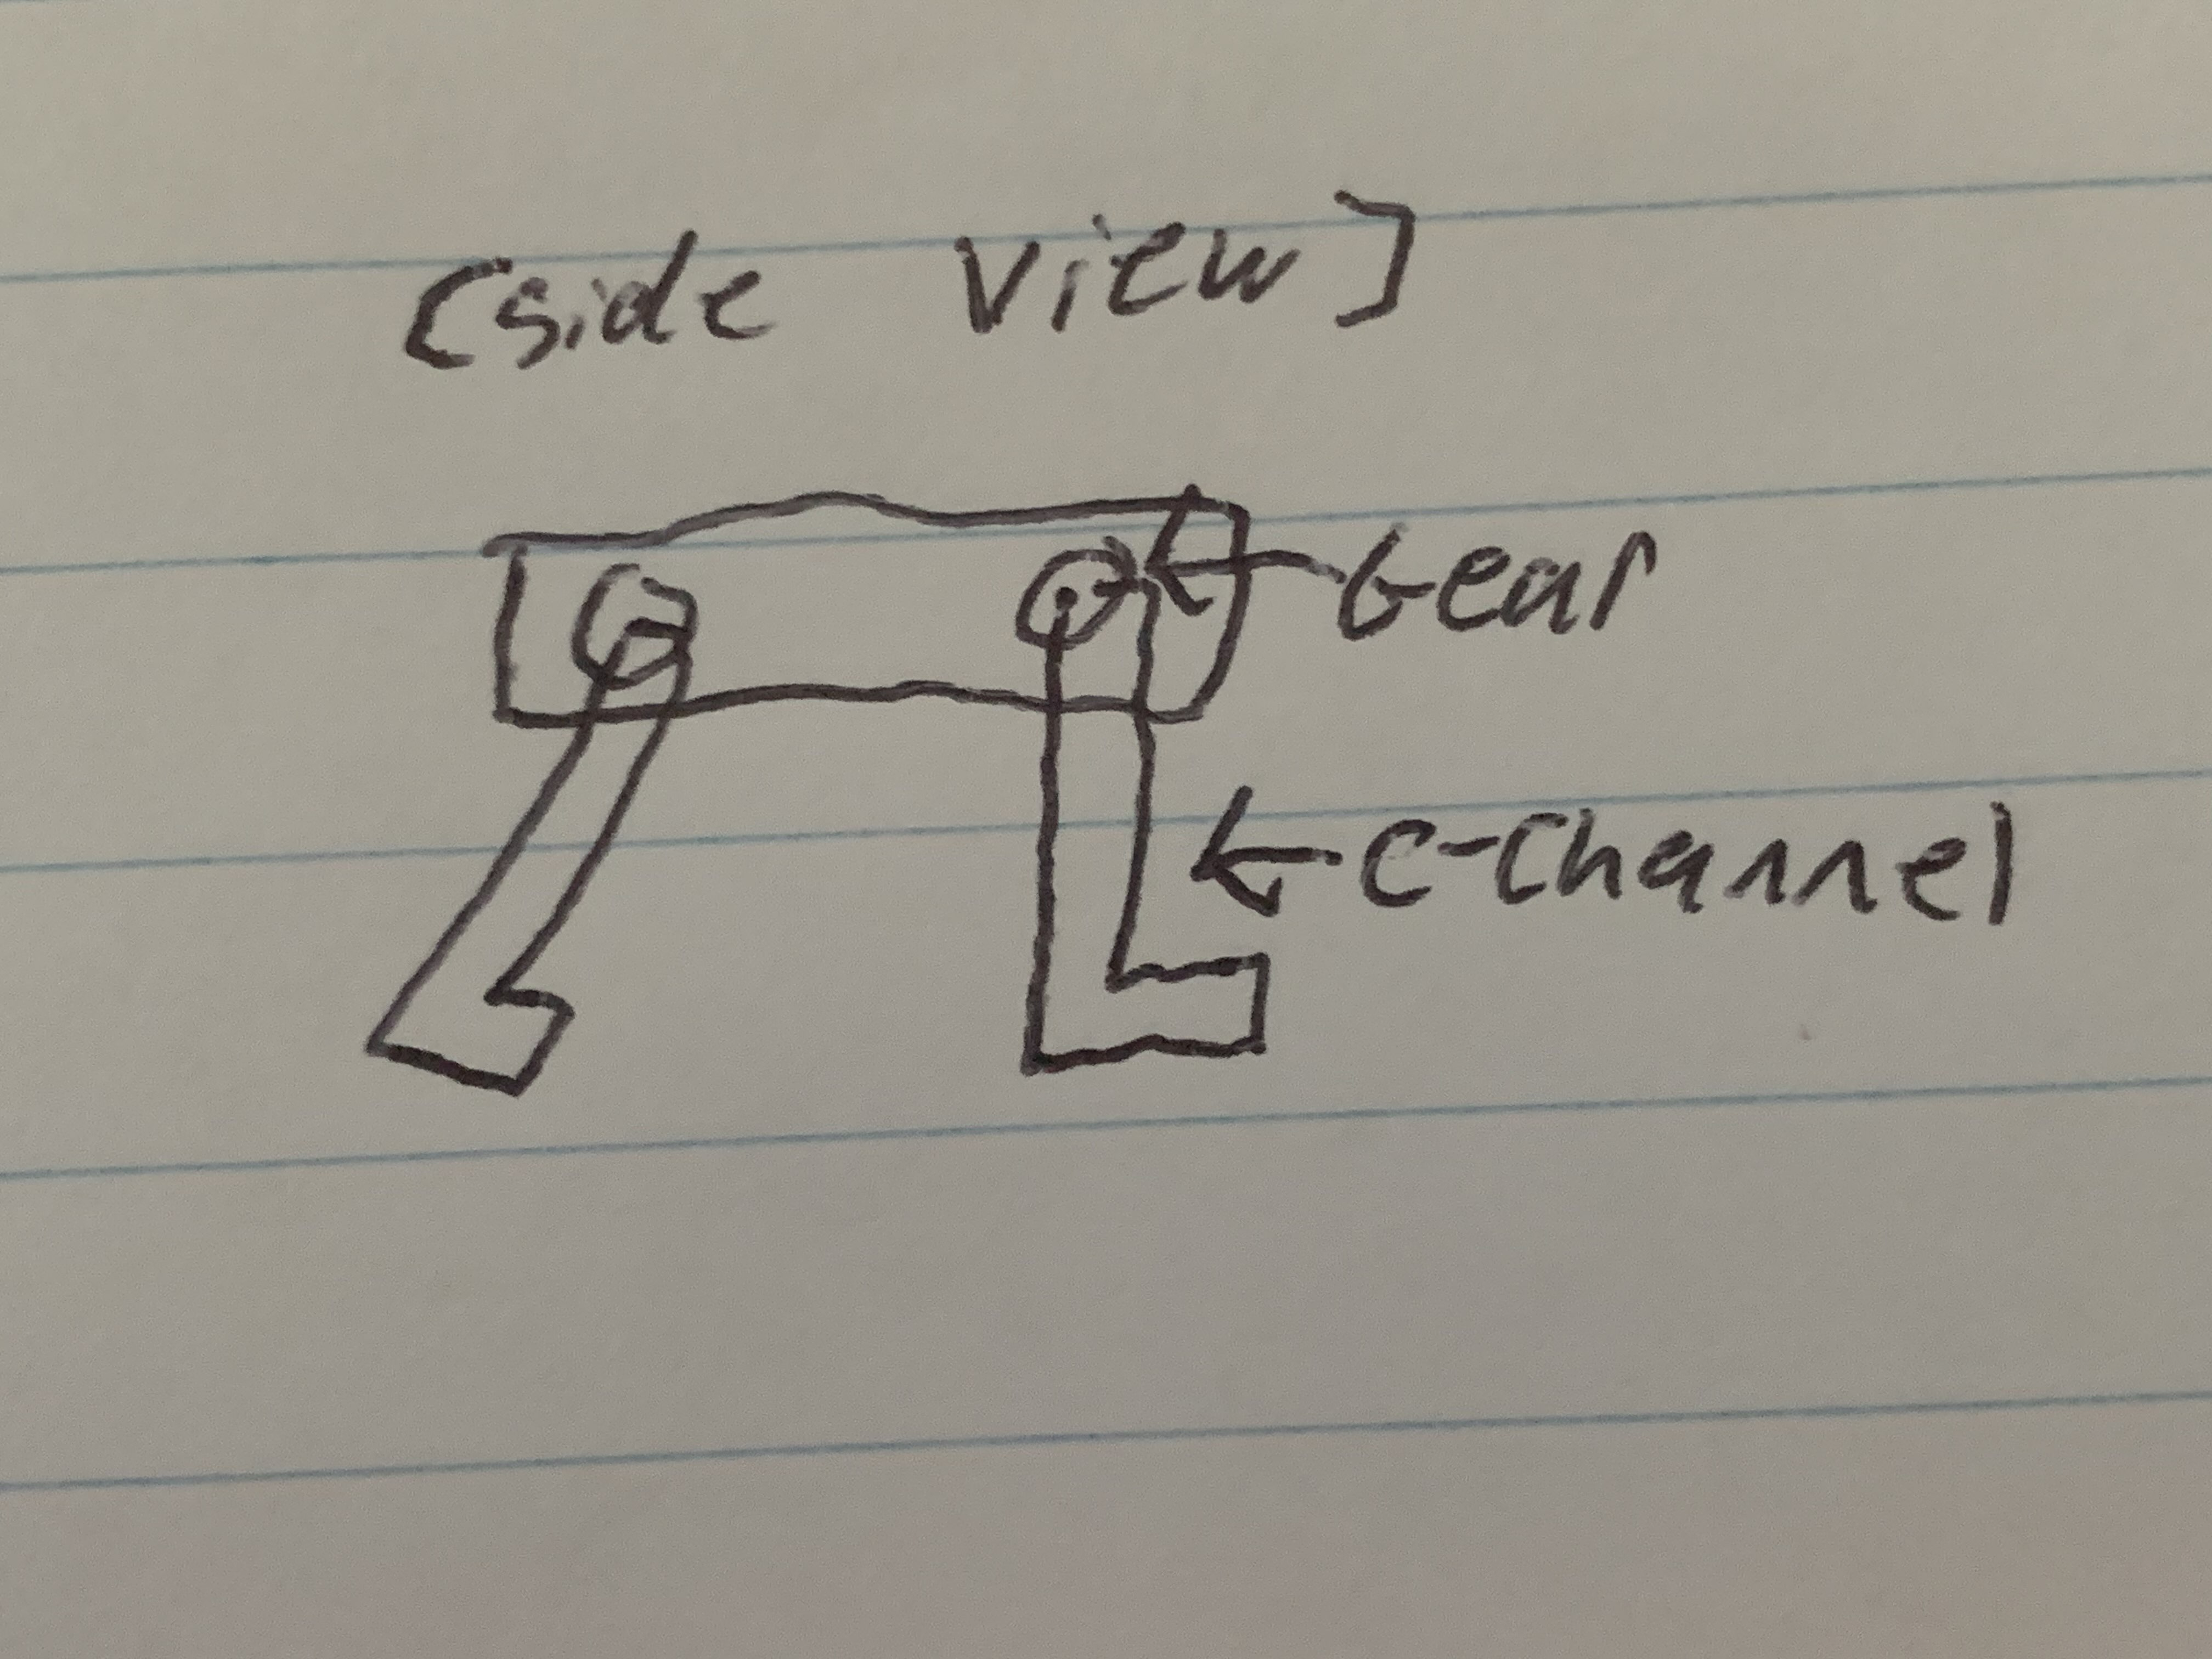
\includegraphics[width=.8\linewidth]{images/Walking Robot.jpg}
        \caption{Walking Robot}
        \label{fig:walking-robot}
    \end{minipage}
\end{figure}
\pagebreak
\white{June 2024}
\begin{center}
    \begin{tikzpicture}
        % Define the dimensions of the calendar
        \def\year{2024}
        \def\month{6}
        \def\monthname{June}
        \def\startday{7} % 1=Sunday, 2=Monday, ..., 7=Saturday
        \def\numdays{30}
        \def\boxwidth{2} % Width of each box
        \def\boxheight{1.8} % Height of each box

\newcommand{\daytext}[1]{
    \ifcase#1
    \or Brainstorm Practice \or \cross  \or \cross \or  Build Practice \or  \cross \or  \cross \or  \cross \or \cross \or  \cross \or \cross
    \or Build Practice \or  \cross \or Build Practice \or  \cross \or Coding Practice \or  \cross \or \cross \or Build Practice \or  \cross \or Build Practice
    \or  \cross \or \cross \or  \cross \or \cross \or Build Practice \or \cross \or Build Practice \or Coding Practice \or \cross \or  \cross
    \or \cross
    \fi
}

        % Draw the calendar grid
        \foreach \x in {0, 1, 2, 3, 4, 5, 6, 7} {
            \draw (\x*\boxwidth, 0) -- (\x*\boxwidth, -6*\boxheight);
        }
        \foreach \y in {0, -1, -2, -3, -4, -5, -6} {
            \draw (0, \y*\boxheight) -- (7*\boxwidth, \y*\boxheight);
        }

        % Add day labels
        \node at (0.5*\boxwidth, 0.5*\boxheight) {Sunday};
        \node at (1.5*\boxwidth, 0.5*\boxheight) {Monday};
        \node at (2.5*\boxwidth, 0.5*\boxheight) {Tuesday};
        \node at (3.5*\boxwidth, 0.5*\boxheight) {Wednesday};
        \node at (4.5*\boxwidth, 0.5*\boxheight) {Thursday};
        \node at (5.5*\boxwidth, 0.5*\boxheight) {Friday};
        \node at (6.5*\boxwidth, 0.5*\boxheight) {Saturday};

        % Add the dates in the top left corner and specific text in the middle
        \foreach \d in {1,...,\numdays} {
            \pgfmathtruncatemacro{\col}{mod(\d+\startday-2, 7)}
            \pgfmathtruncatemacro{\row}{-(\d+\startday-2)/7}
            \node[anchor=north west] at (\col*\boxwidth, \row*\boxheight) {\d};
            \node[anchor=center, text width=\boxwidth cm, align=center] at (\col*\boxwidth+0.5*\boxwidth, \row*\boxheight-0.5*\boxheight) {\daytext{\d}};
        }

        % Add month and year
        \node at (3.5*\boxwidth, 1.5*\boxheight) {\textbf{\monthname\ \year}};
    \end{tikzpicture}
\end{center}
This is our what happened during the month of June. We had full team meetups every Tuesday and every Thursday except for June the 6th. Connor had the robot during this time, Ian has been working on the AI, and Jayden has been working on the simulator, which will have a full chapter on it once in place. At the end of the month we had just finished the Clamp. 
\solution{Choose a Solution \& Make a Plan: Drivetrain (June 3, 2024}
\label{Choose-a-Solution-&-Make-a-Plan:-Drivetrain}
\chapterauthor{Caleb Bachmeier}
\info{Caleb Bachmeier}{Choose a Solution \& Make a Plan: Drivetrain}{June 3, 2024}
\textbf{Goal}: Choose which solution to use for our drivetrain
    \section*{Choose a Solution}
\subsection*{Decision Matrix}
On the following page is a (\blueref{tab:drive-matrix}{decision matrix}). A decision matrix, also known as a decision-making grid, is a systematic tool used to evaluate and prioritize a set of options based on a predefined set of criteria. It's particularly useful in engineering and other technical fields where decisions often involve weighing multiple factors or criteria. Which is why we've decided to use one to decide which type of drive to use. The team has already ruled out Mecanum, X-Drive, Tank Treads, and Walking Robot because we've never seen any top teams use those types of drives. The row "Weight" determines how much weight a specific column revives in terms of points. It wouldn't be fair to compare the size of the robot and the speed 1-1 because speed is much more important than size.
\pagebreak
\renewcommand{\arraystretch}{1.85} % Change this value as needed
\begin{table}[htb!]
\centering
\begin{tabular}{|>{\centering\arraybackslash}m{1.85cm}|>{\centering\arraybackslash}m{1.85cm}|>{\centering\arraybackslash}m{1.85cm}|>{\centering\arraybackslash}m{1.85cm}|>{\centering\arraybackslash}m{1.85cm}|>{\centering\arraybackslash}m{1.85cm}|>{\centering\arraybackslash}m{1.85cm}|}
\hline
\textbf{Scale 1 - 10} & \textbf{Complexity} & \textbf{Motors Needed} & \textbf{Traction} & \textbf{Size} & \textbf{Speed} & \textbf{Total} \tabularnewline
\hline
Weight & x1 & x3 & x2 & x1 & x3 & \tabularnewline
\hline
Standard Omni & 10 & 10 & 6 & 10 & 6 & 88 \tabularnewline
\hline
Omni and Traction & 10 & 10 & 10 & 10 & 8 & 94 \tabularnewline
\hline
Traction & 10 & 10 & 10 & 10 & 4 & 74 \tabularnewline
\hline
H-Drive & 6 & 8 & 6 & 10 & 6 & 70 \tabularnewline
\hline
\end{tabular}
\caption{Drive Decision Matrix}
\label{tab:drive-matrix}
\end{table}
\renewcommand{\arraystretch}{1.85} % Reset to default

Looking at the point totals, it seems that a Omnidirectional and Traction wheel drive is our best option.
\subsection*{Brainstorm}
Using a Traction and Omnidirectional wheel drive, our initial design incorporated a 600 RPM drive with 2.75-inch wheels, which satisfied our baseline speed criteria. However, a subsequent CAD analysis indicated that the 36-tooth gears in our original gearing arrangement resulted in insufficient spacing for idler gears due to the proximity of the wheels (\blueref{fig:600-RPM-clearance-issue}{600 RPM Clearance Issue}). In search of alternatives, we contemplated utilizing 48-tooth gears, but this adjustment extended the drive beyond our 15-inch maximum length constraint (\blueref{fig:48t-gears-=-too-long}). We then explored a 450 RPM drive with 2.75-inch wheels, which improved wheel spacing, but this configuration fell short of our velocity target, achieving only 64 inches/second—just below our 65 inches/second minimum threshold (\blueref{fig:450-on-3.25-issue}{450 RPM on 3.25 inches issue}). A switch to 3.25-inch wheels rectified the speed shortfall, but reintroduced the clearance problem encountered earlier.


\begin{center}
    \textbf{These are some are computer aided designs (CAD) using Fusion 360 of the problems listed above}
\end{center}
\begin{figure} [htb!]
    \begin{minipage}{.5\textwidth}
        \centering
        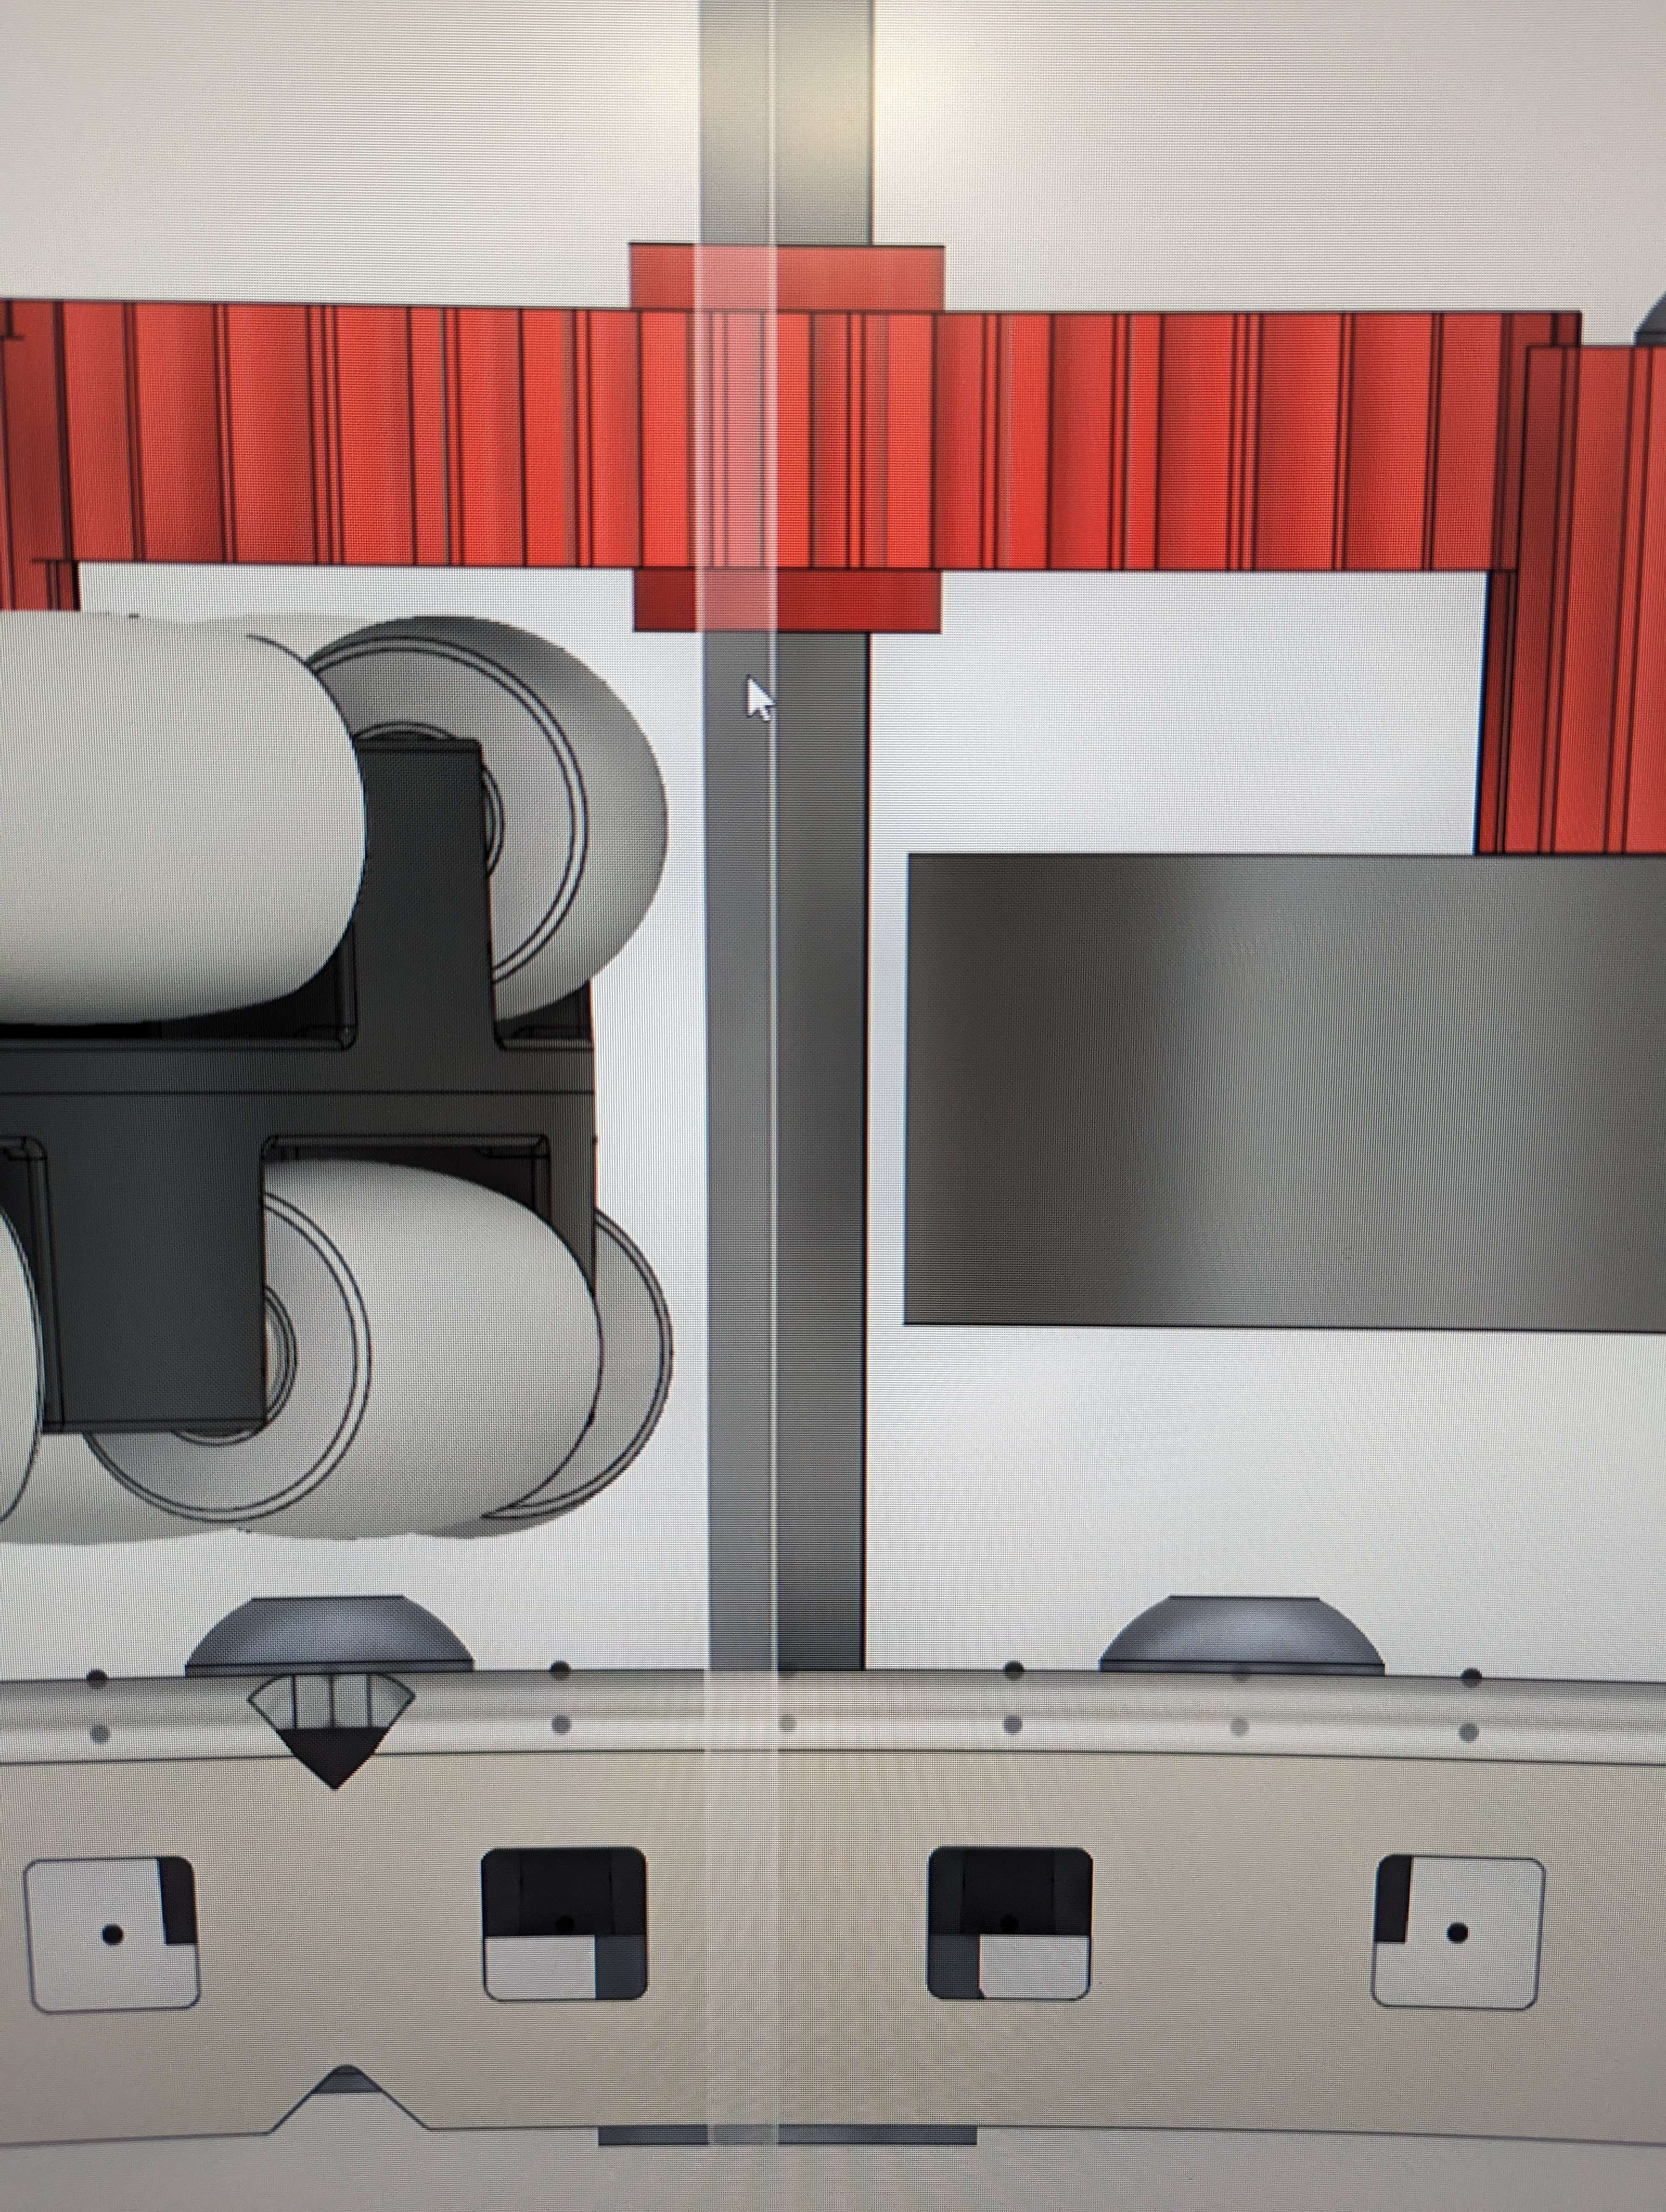
\includegraphics[width=.8\linewidth]{images/600 RPM Clearance Issue.jpg}
        \caption{600 RPM Clearance Issue}
        \label{fig:600-RPM-clearance-issue}
    \end{minipage}
    \begin{minipage}{.5\textwidth}
        \centering
        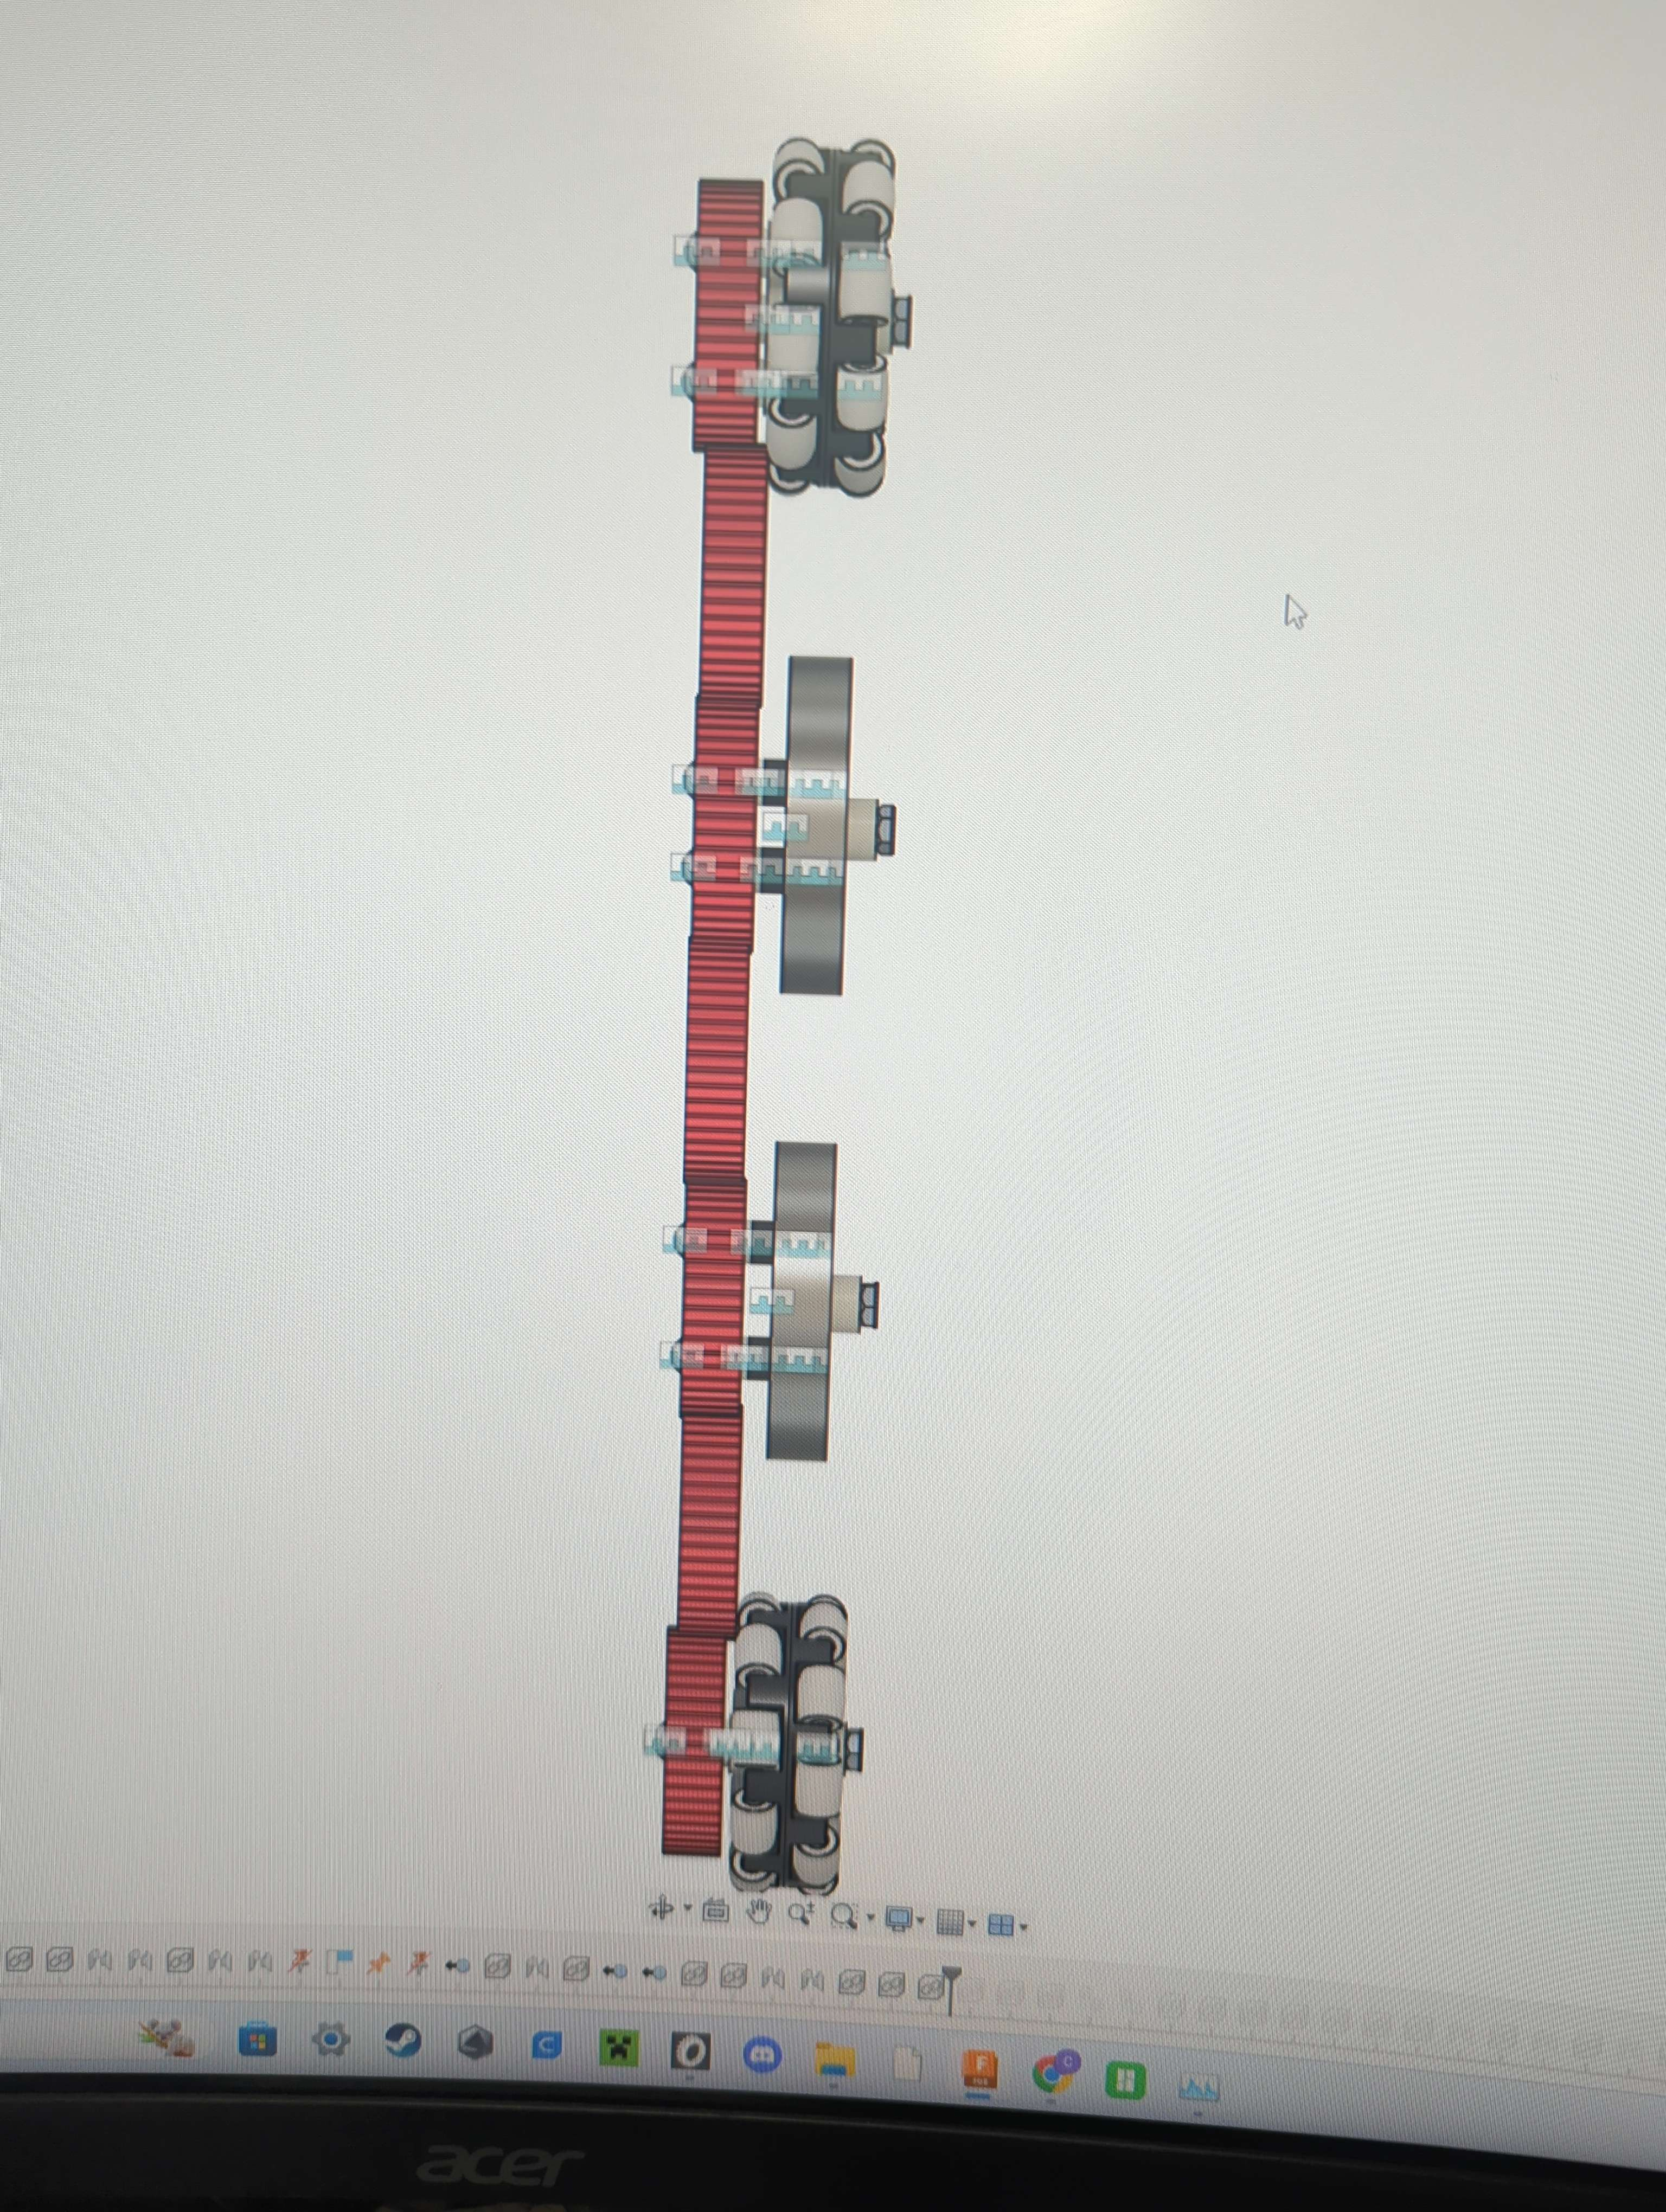
\includegraphics[width=.8\linewidth]{images/48t gears = too long.jpg}
        \caption{48 Tooth Gears}
        \label{fig:48t-gears-=-too-long}
    \end{minipage}
    \begin{minipage}{.5\textwidth}
        \centering
        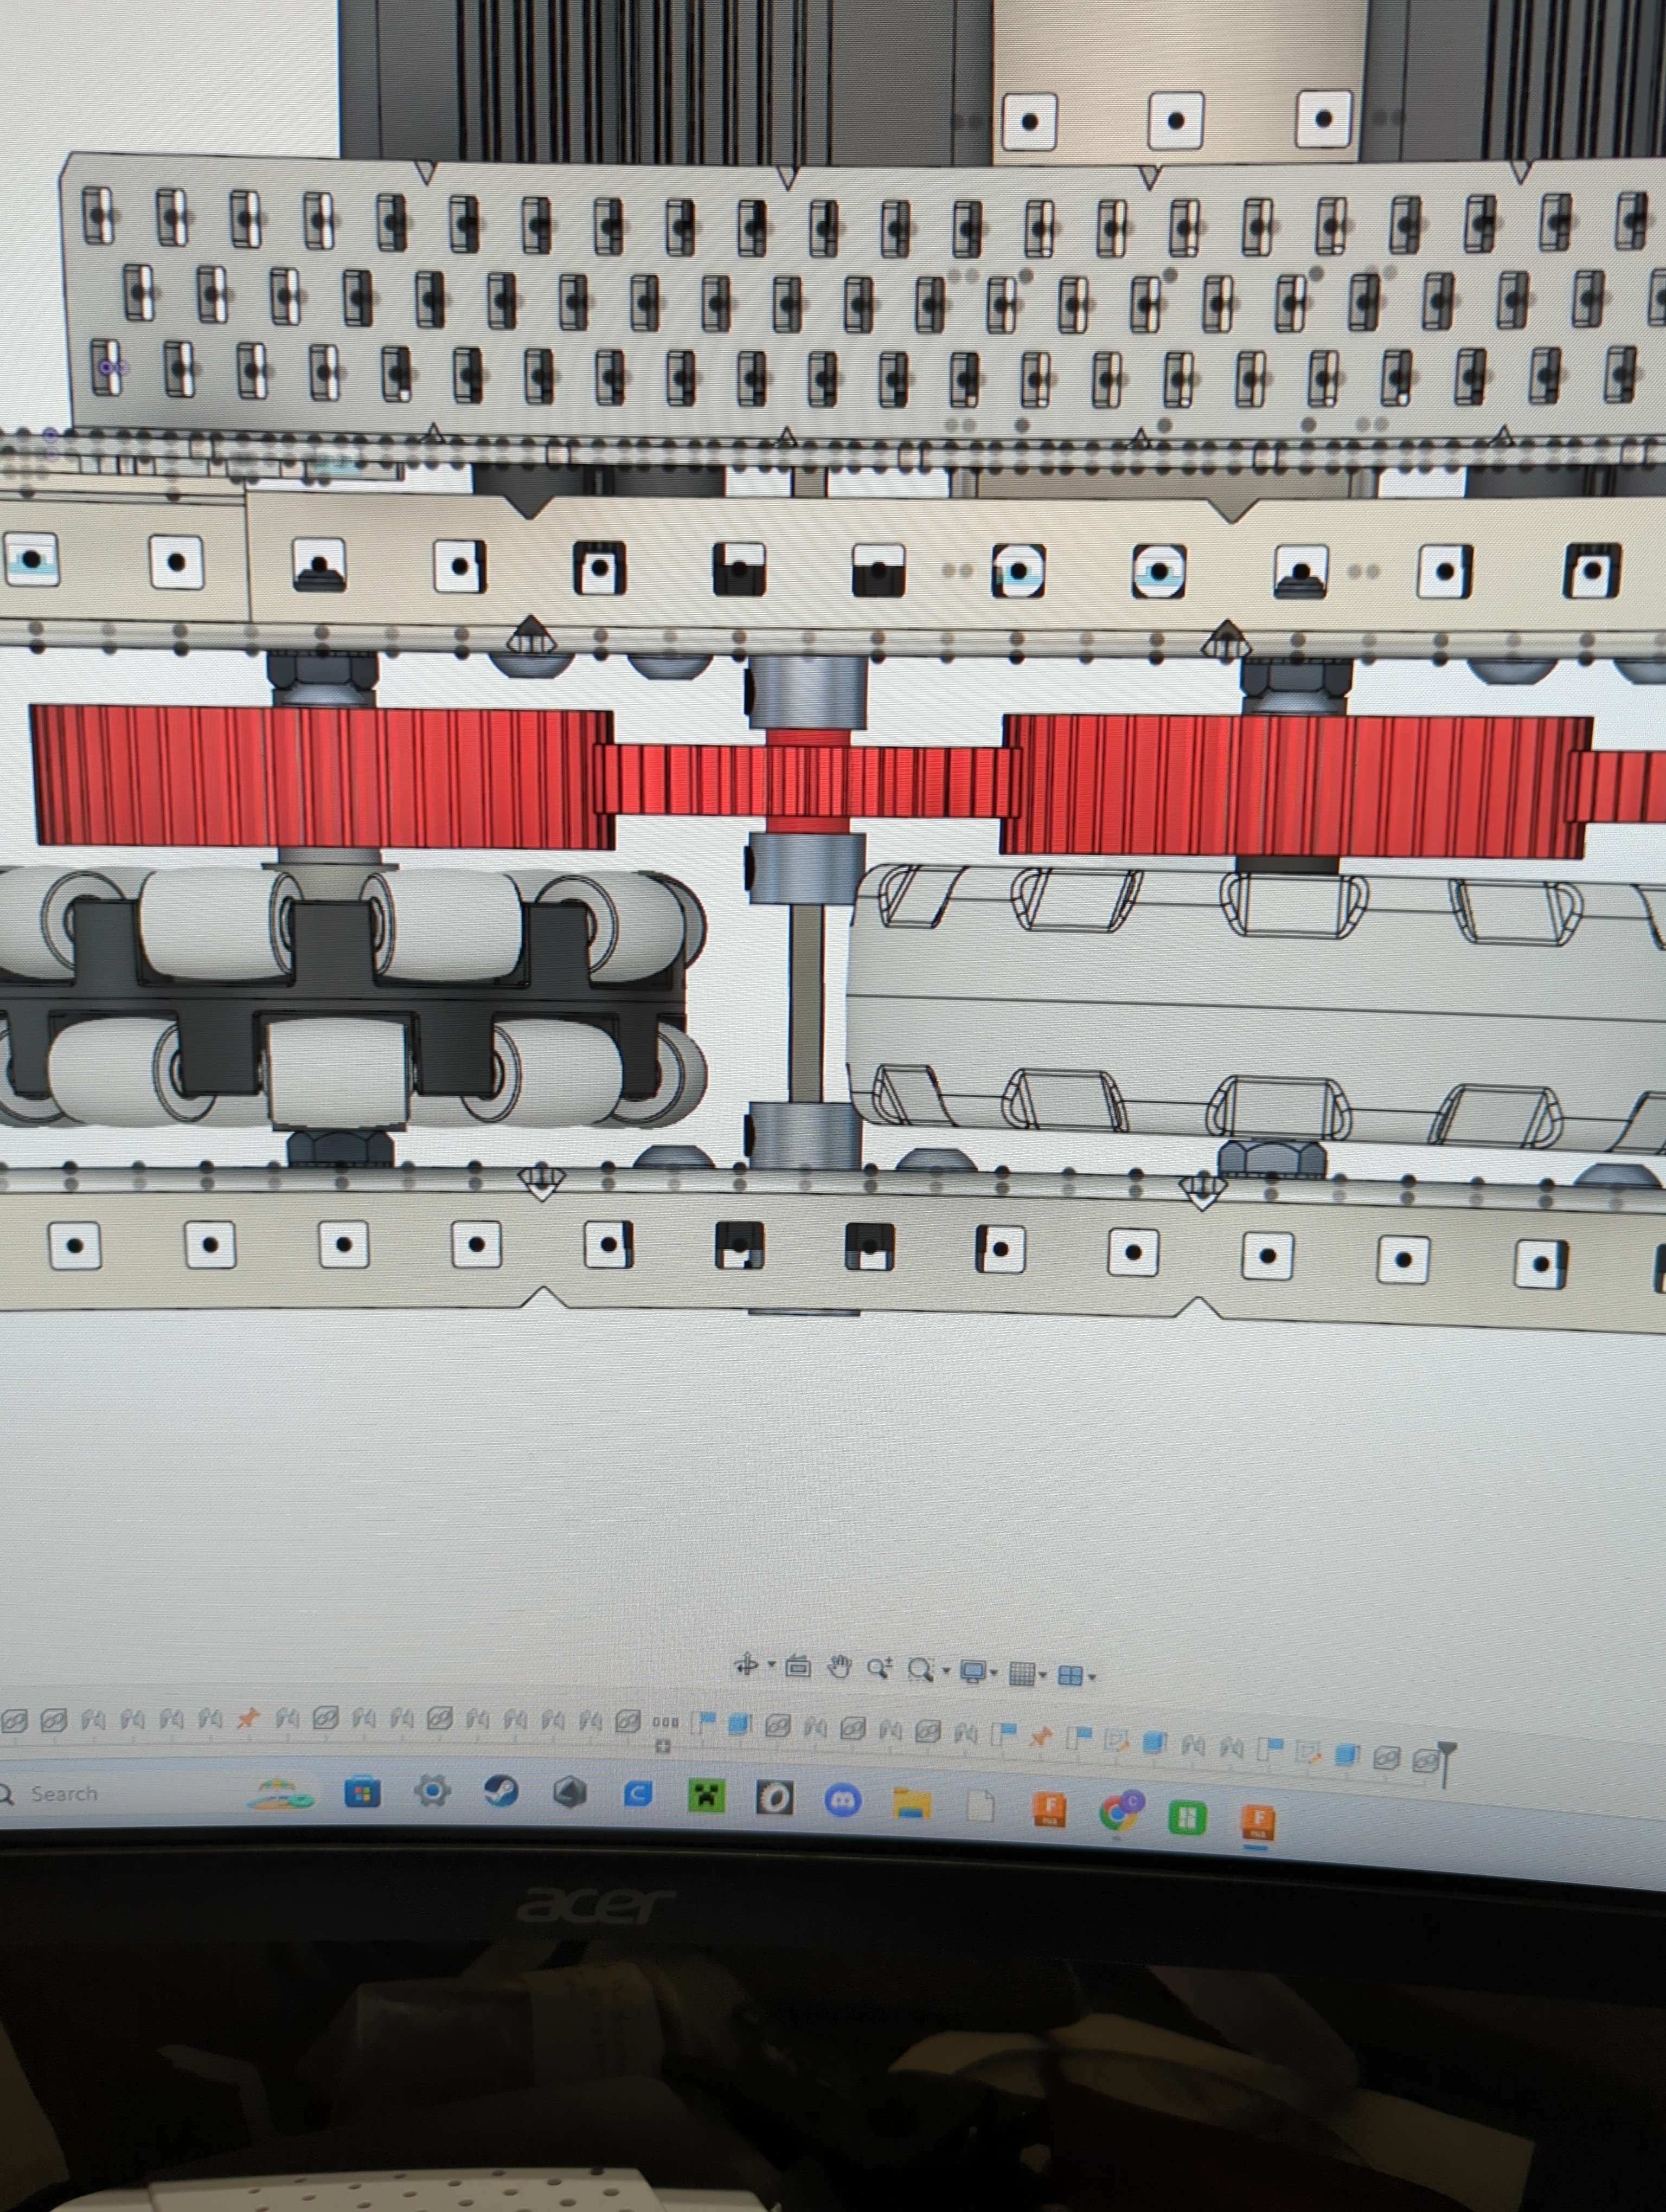
\includegraphics[width=.8\linewidth]{images/450 on 3.25 issue.jpg}
        \caption{450 Rpm Clearance Issue}
        \label{fig:450-on-3.25-issue}
    \end{minipage}
\end{figure}
Ultimately, we settled on a 480 RPM drive with 3.25-inch wheels. This final iteration successfully conformed to our dimensional limit, measuring approximately 14.75" in length, and surpassed our speed requirement with a peak velocity of 82 inches/second. Our wheel arrangement incorporated both, traction and omni wheels in order to overcome the disadvantages of both. by placing a traction wheel in the middle of each side of the drive with omni wheels at the front and rear of it, we overcome the poor turning of the traction wheel by turning it into a pivot and by having a traction wheel at all, we significantly increase our resistance to side pushes. 
\pagebreak
\subsection*{CAD}
Below are the complete CAD designs of our planned drivetrain
\begin{figure}[hbt!] % Use [hbt!] to place the figures on the same page
    \begin{minipage}{.5\textwidth}
        \centering
        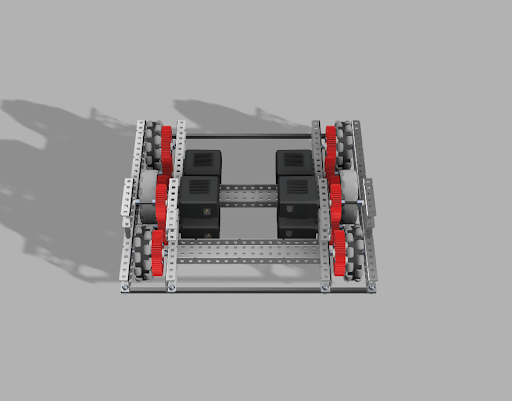
\includegraphics[width=.8\linewidth]{images/Frontdown-V1-Drivetrain.png}
        \caption{Front view}
        \label{fig:frontdown}
    \end{minipage}
    \begin{minipage}{.5\textwidth}
        \centering
        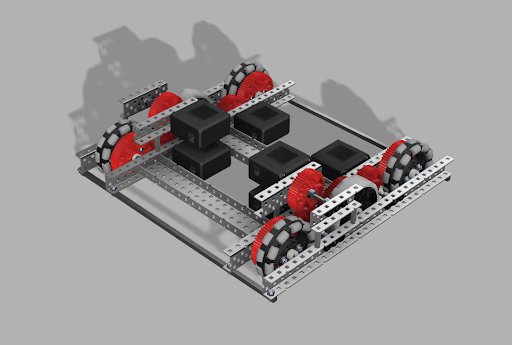
\includegraphics[width=.8\linewidth]{images/Iso-V1-Drivetrain.png}
        \caption{Isometric view}
        \label{fig:iso}
    \end{minipage}
    \begin{minipage}{.5\textwidth}
        \centering
        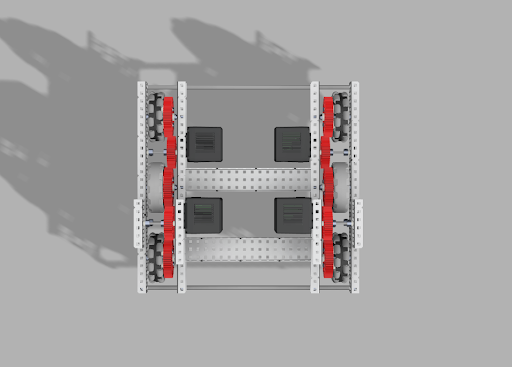
\includegraphics[width=.8\linewidth]{images/Topdown-V1-Drivetrain.png}
        \caption{Top view}
        \label{fig:topdown}
    \end{minipage}
    \begin{minipage}{.5\textwidth}
        \centering
        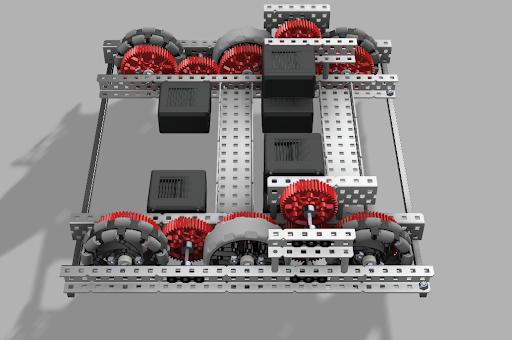
\includegraphics[width=.8\linewidth]{images/Sidedown-V1-Drivetrain.png}
        \caption{Side view}
        \label{fig:sidedown}
    \end{minipage}
\end{figure}

This is our complete CAD for our drivetrain. We always CAD out projects before we build them, so we can see any problems with our potential solution. We decided on 480 RPM using 3.25-inch wheels, measuring approximately 14.75" in length. This will have the velocity of 82 inches/seconds. We see no problems, so we are ready to start building.


\build{Build \& Program: Drivetrain (June 5, 2024)}
\label{Build-&-Program:-Drivetrain}
\chapterauthor{Connor Albers}
\info{Caleb Bachmeier}{Build \& Program: Drivetrain}{June 5, 2024}
\textbf{Goal}: Build \& program our selected drivetrain
    \section*{Building}
\subsection*{Cutting the Drive Rails}
To construct our drive we began by cutting the four "drive rails" to a length of 27 holes; this provided space for our gearing with an extra hole on the front and back of the drive to give room for additional support.
\begin{figure}[h]
    \begin{minipage}{.5\textwidth}
        \centering
        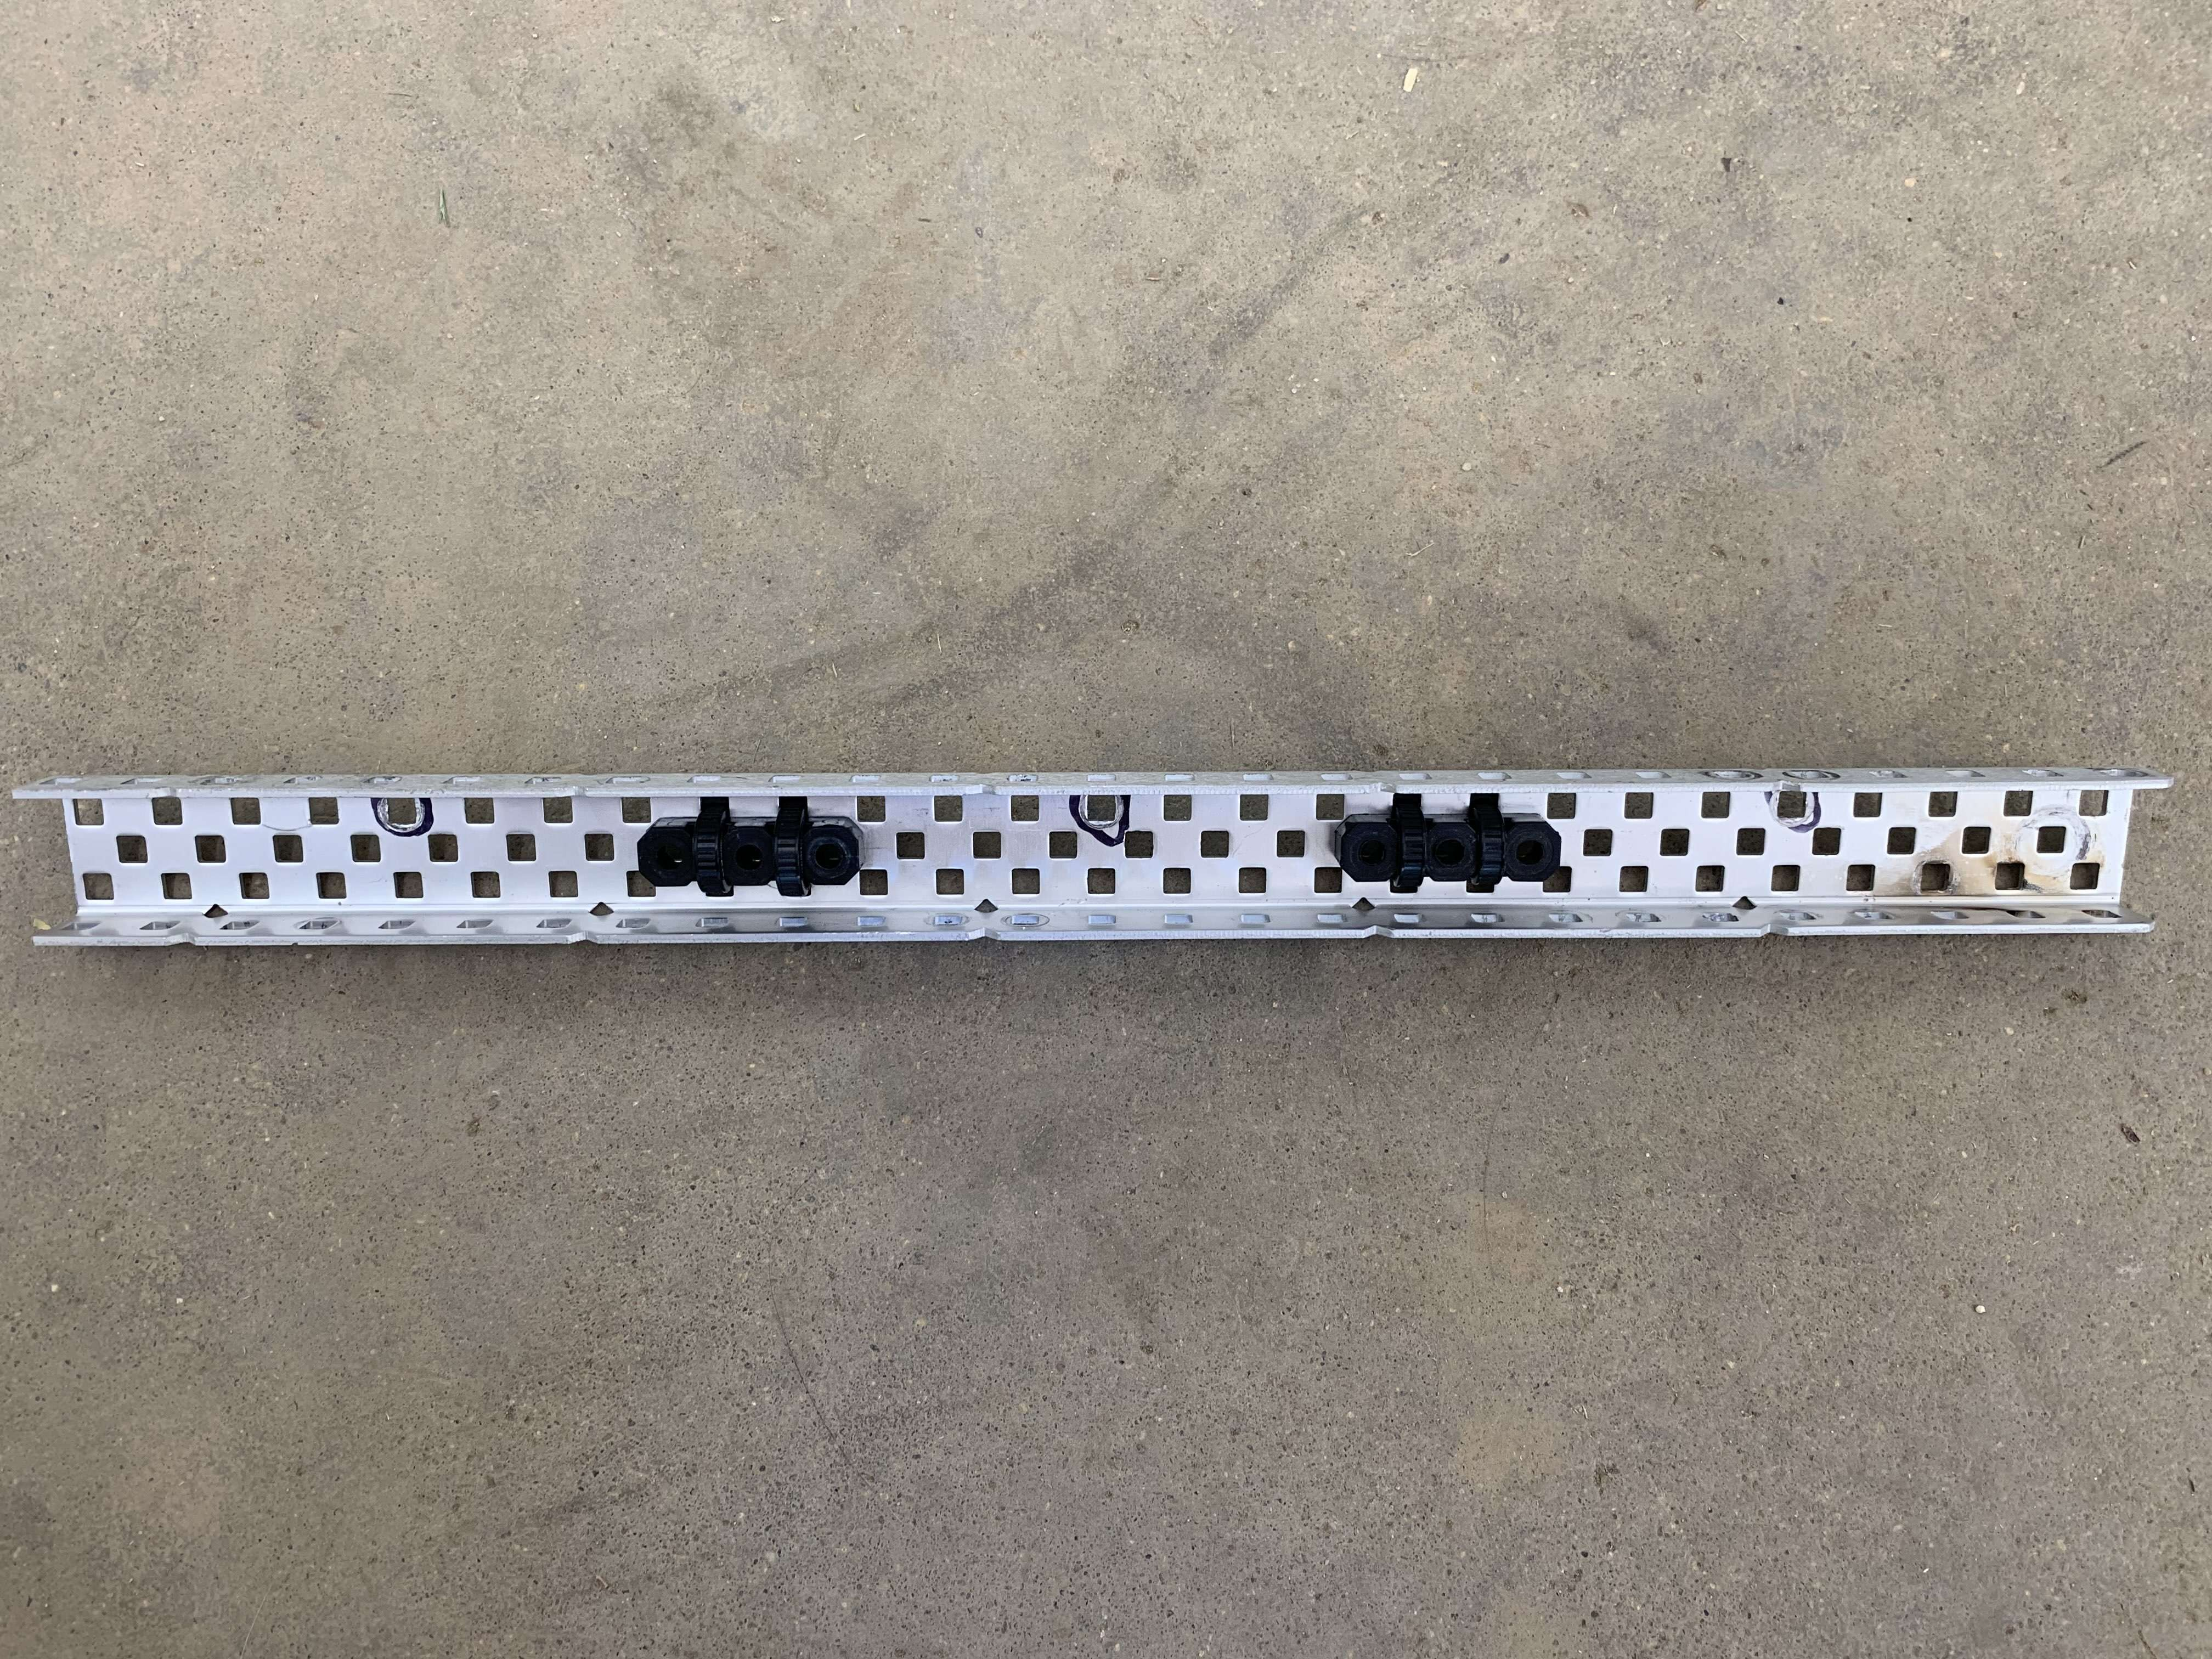
\includegraphics[width=.8\linewidth]{images/C Channel w zipties.jpg}
        \caption{Drive Rail}
        \label{fig:c-chanell-w-zipties}
    \end{minipage}
    \begin{minipage}{.5\textwidth}
        \centering
        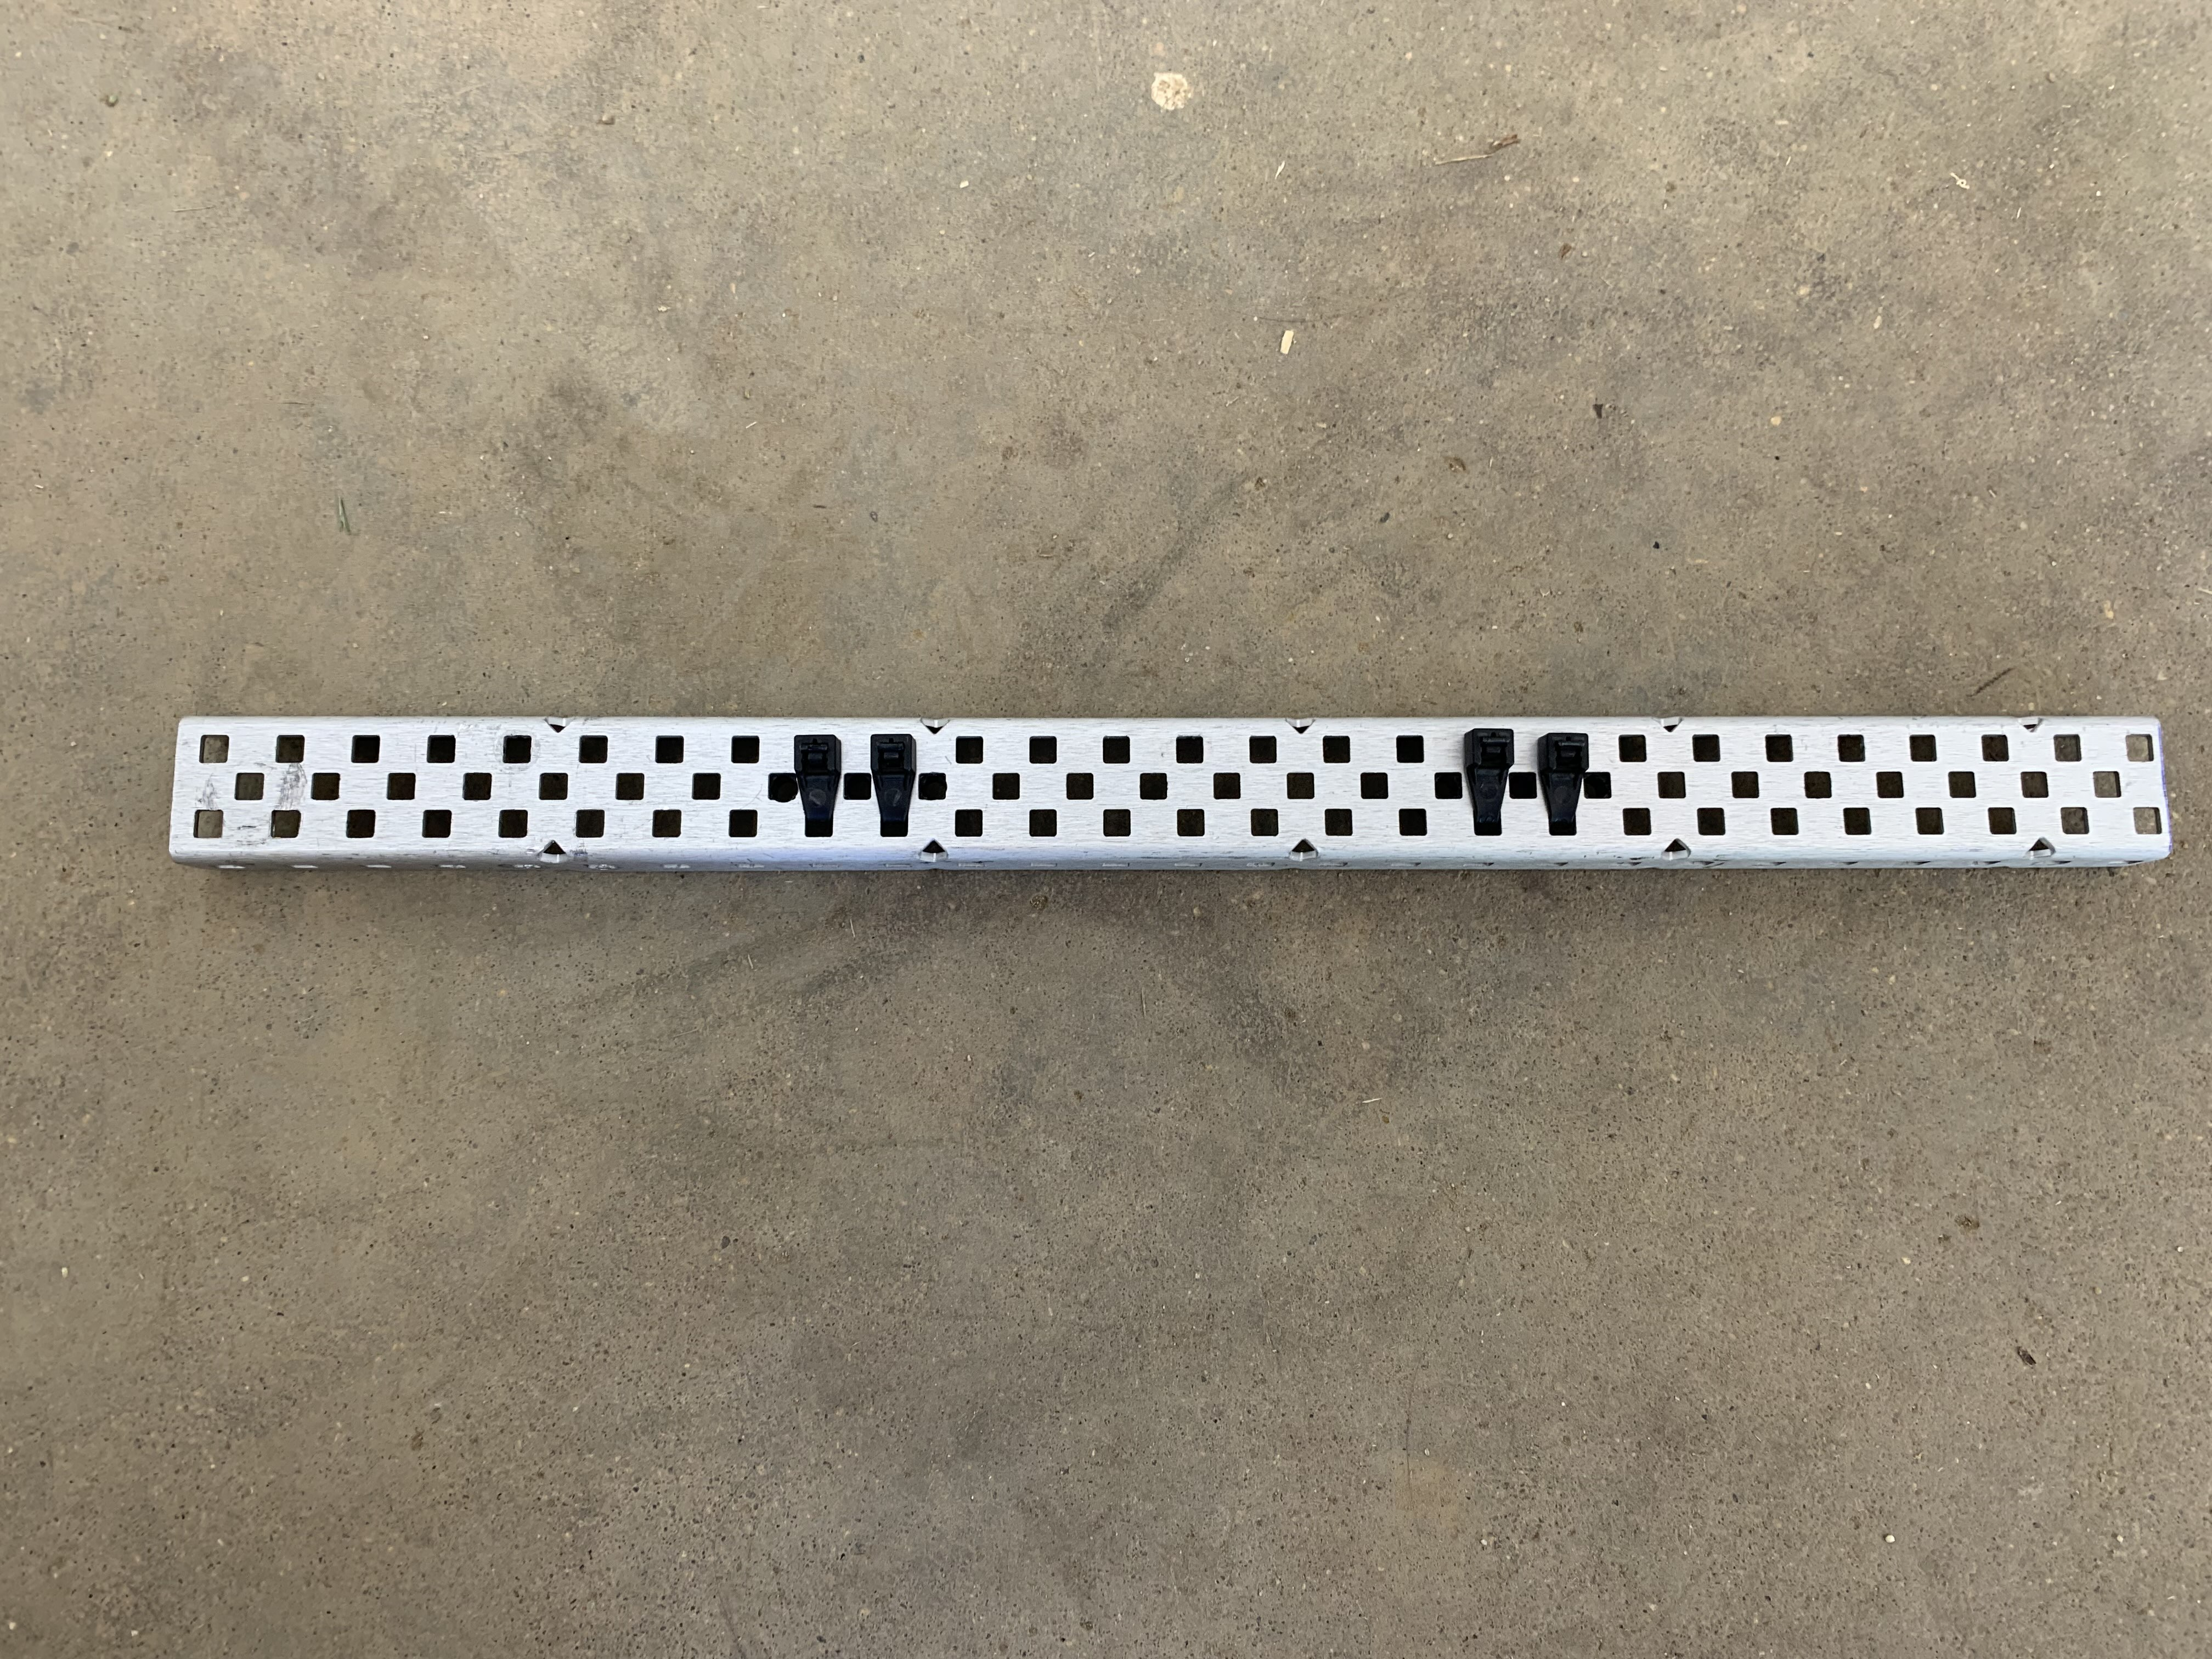
\includegraphics[width=.8\linewidth]{images/Other side of Drive Rail.jpg}
        \caption{Opposite Side of Drive Rail}
        \label{fig:opposite-side-of-drive}
    \end{minipage}
\end{figure}
\subsection*{Zip Tie Bearings}
Our next step was to zip tie the 2 bearings per rail that the idlers gears require. The use of zip tie bearings saves large amounts of weight ultimately contributing to larger acceleration and top speed as well as maneuverability. The bearings are evenly spaced on the the middle row of our 1x2 c-channel drive rails; providing the correct spacing for our gearing.

\subsection*{Adding Screws}
Our next step was to add the 3 screws per side of the drive for the screw joints for the wheels on the bottom row of the drive rails. It is important to note that we inserted the screws into the rails that would end up on the exterior of our drive in order to ensure that we would have access to the screws should we need to tighten any aspect of the joint. After inserting the 2.5" long screws, we threaded lock nuts all the way down the threaded region, effectively turning them into studs. After adding the studs we added 1/4" spacers to all of the studs to prevent the wheels rubbing on the rails; they would rub due to the hubs of the wheels being inset from tread of the wheels.

\subsection*{Constructing Wheel Sub Assemblies and Properly Spacing Them Within the Drive}
Before we could continue the the main build we needed to construct the wheel sub assemblies. While we did have multiple types of wheels, traction and omnidirectional, the process of construction remained the same. The process consisted of using 2 bolts to attach a 60t HS v2 gear to the hub of the wheel with 1/4" spacers in between. Using v2 HS gear removes the need for additional spacers (this is better explained in \blueref{fig:v1-and-v2-gears}{V1 and V2 gears}). After inserting 2 brass circle inserts per wheel, we slid the wheels onto the the screw with the side without the gear facing to what was to be the outside of the drive. Following the wheels, we added 1/8" spacer to each stud; this ensured the spacing between our inside drive rail and outside drive rail was divisible by 1/2"; thus, cohering with the VEX grid system; thence, allowing us to add structure across the drive rails without needing to drill custom holes. The proceeding step was tightening lock nuts on all of the studs to the point where they are as tight as they can be while still allowing the wheels to spin freely. Next we added the second rail to each side followed by a final nut on the end of each study, this time tightening the nut all the way.
\begin{figure}[h!] % Use [hbt!] to place the figures on the same page
        \centering
        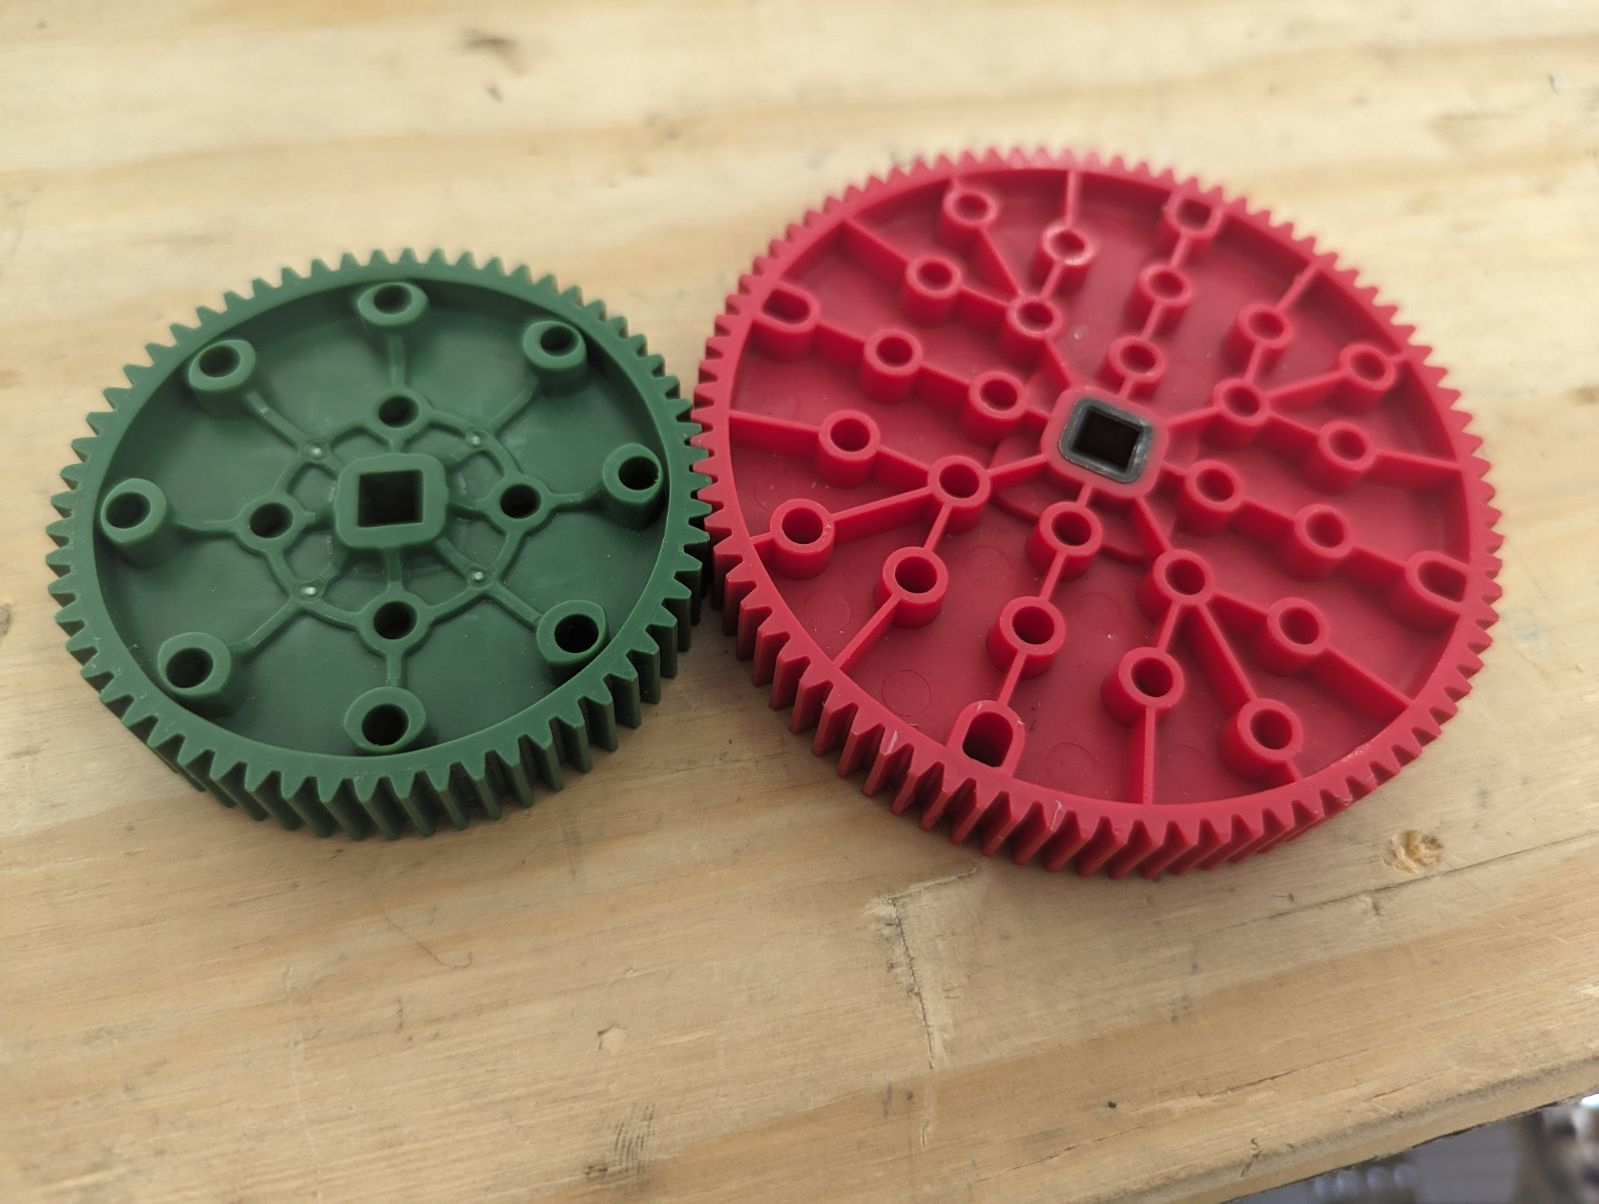
\includegraphics[width=.8\linewidth]{images/V1 and V2 Gears.jpeg}
        \caption{V1 and V2 Gears}
        \label{fig:v1-and-v2-gears}
\end{figure}


\subsection*{Inserting Motor Screws}
The next step was to insert the motor screws as we will not be able to insert them after adding idler gears. This is a very simple step in assembling any VEX component; unfortunately due to spacing issues we were only able to get 1 screw in each motor as opposed the more secure 2. While using only 1 screw per motor is generally not a good idea, we found that by using only 1 screw we can quickly swap motor by inserting our screwdriver through the holes in the outer rail and through the 48t idle gears that are later added.

\subsection*{Adding Idler Gears and Motors}
After cutting 4 shafts to a length of around 3", the next step was to add the shafts for the idler gears, two per side. For specific details on the hardware and spacers used check \blueref{fig:idler-gears}{Idler Gears}. The final step was to add the motors with the addition of steel inserts to ensure the motor gripped the shafts effectively.
\begin{figure}[b]
    \centering
    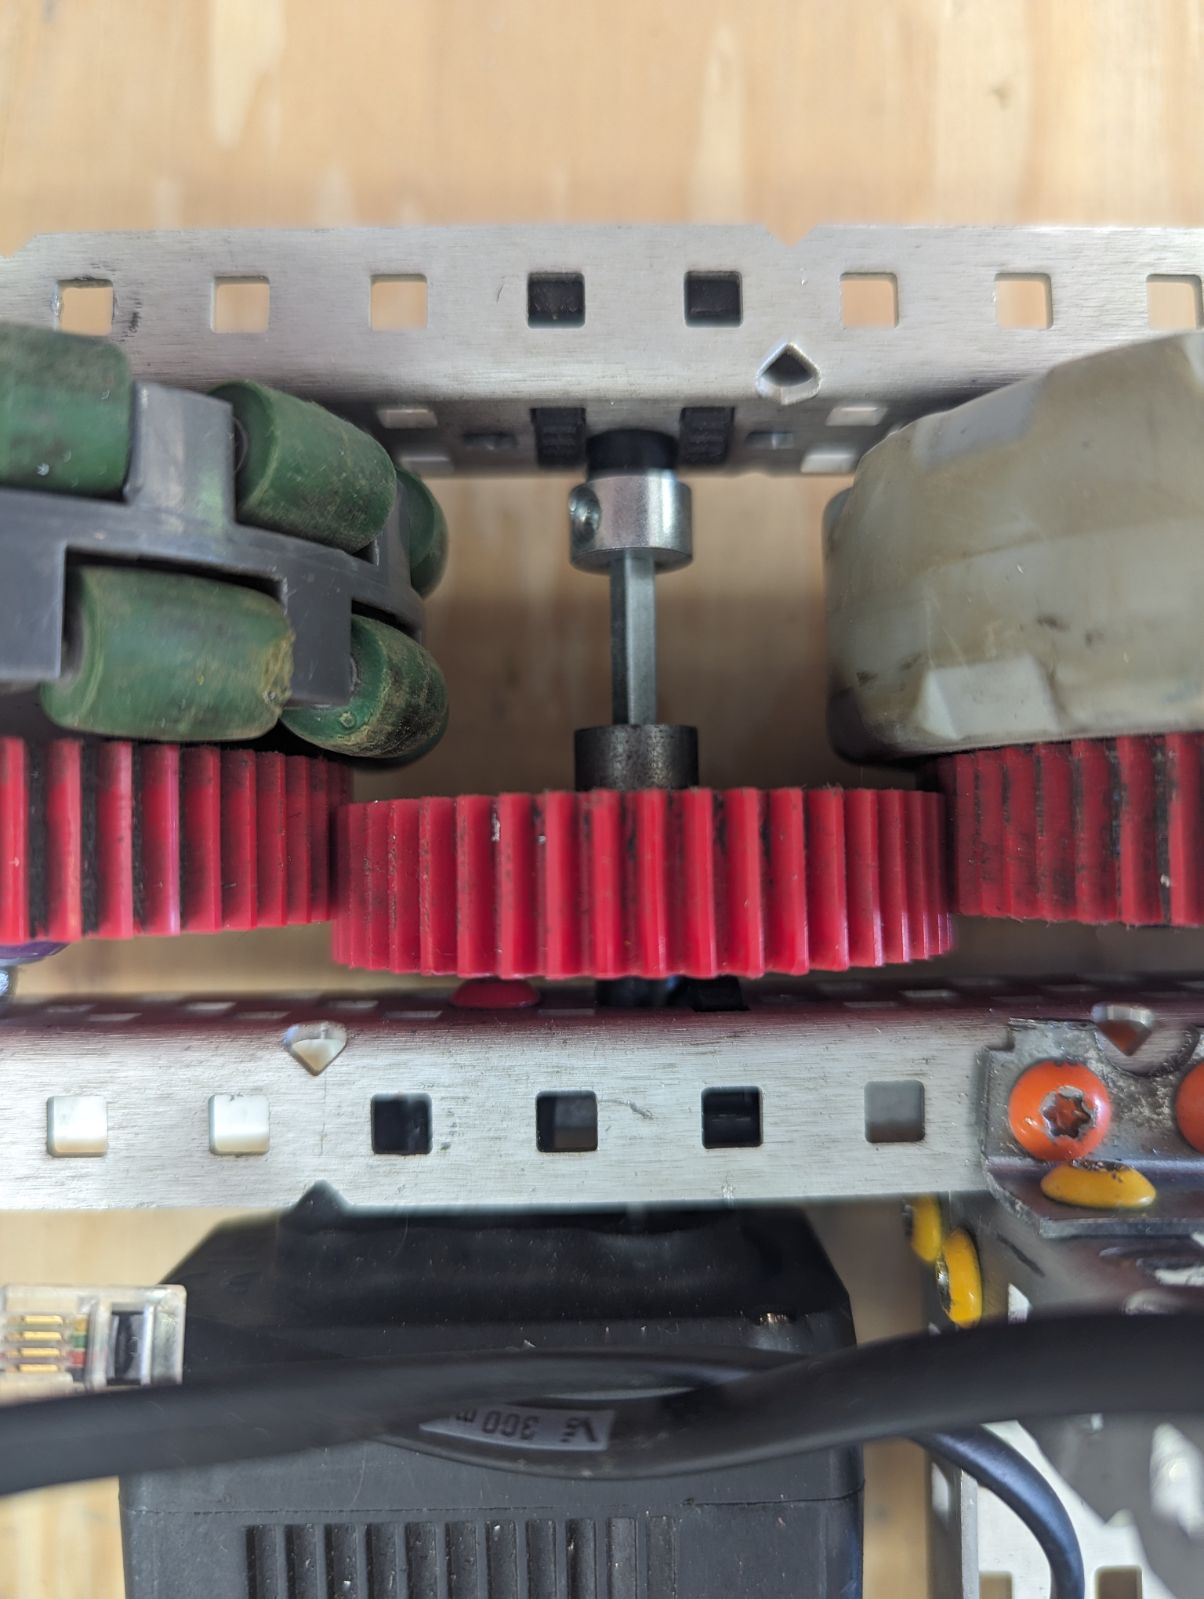
\includegraphics[width=0.5\linewidth]{images/Idler Gears.jpeg}
    \caption{Idler Gears}
    \label{fig:idler-gears}
\end{figure}

\subsection*{Motor Towers}
The current setup only featured a total of four motors but we wanted our final drive to have six. The solution: motor towers. Motor towers are commonly used when a compact motor layout is required or, like in our case, there are too few idle gear axles to add the desired number of motors. Motors towers involve gearing a motor into the drive from above rather that directly into the drive. Our motor towers feature the exact same construction as our idle gears with the only change being that they are moved above the wheels rather than beside them with the help of some 1x5 c-channels that were cut at a length of 5 holes. The use of 1x5 C-Channel provided extra mounting locations should we need them in the future.

\subsection*{Assembling the Drivetrain}
After completing both individual sides of the drive we had to conquer the task of assembling them to be one complete drivetrain. The solution we chose for this was high strength axles. The use of high strength axles provides our drive with copious amounts of strength while remaining low profile so as not to get in the way of other, future mechanisms. Unfortunately using high strength axles, as opposed to c-channel, means we must drill out every point we wish to attach to. This was simply unpractical for anything beyond attaching the sides of the drivetrain together. Our approach to this problem included using high strength axles that spanned the entire width of the drive and using shorter c-channels that only spanned to the inter lip of each side of the drive. This is better explained in \blueref{fig:mounting-rails-hs-axles}{Mounting rails with high strength axles}. After mounting just 1 high strength axle at both the front and rear of the drive, our drive turned out to be surprisingly rigid -- being the most rigid drive we had ever built.
\begin{figure}[h]
    \centering
    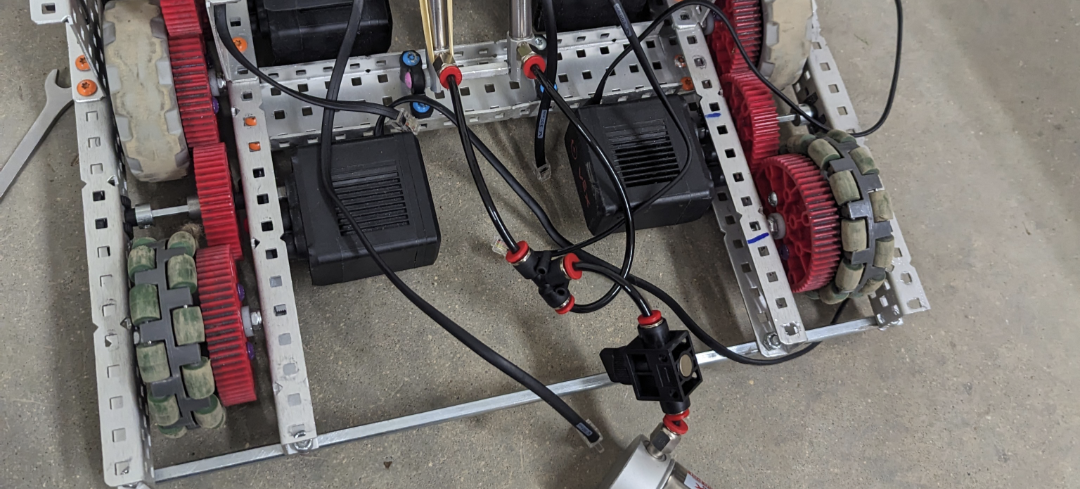
\includegraphics[width=1\linewidth]{images/Mounting Rails HS Axles.png}
    \caption{Mounting the Rail}
    \label{fig:mounting-rails-hs-axles}
\end{figure}
\begin{figure} [hbt!]
    \begin{minipage}{.5\textwidth}
        \centering
        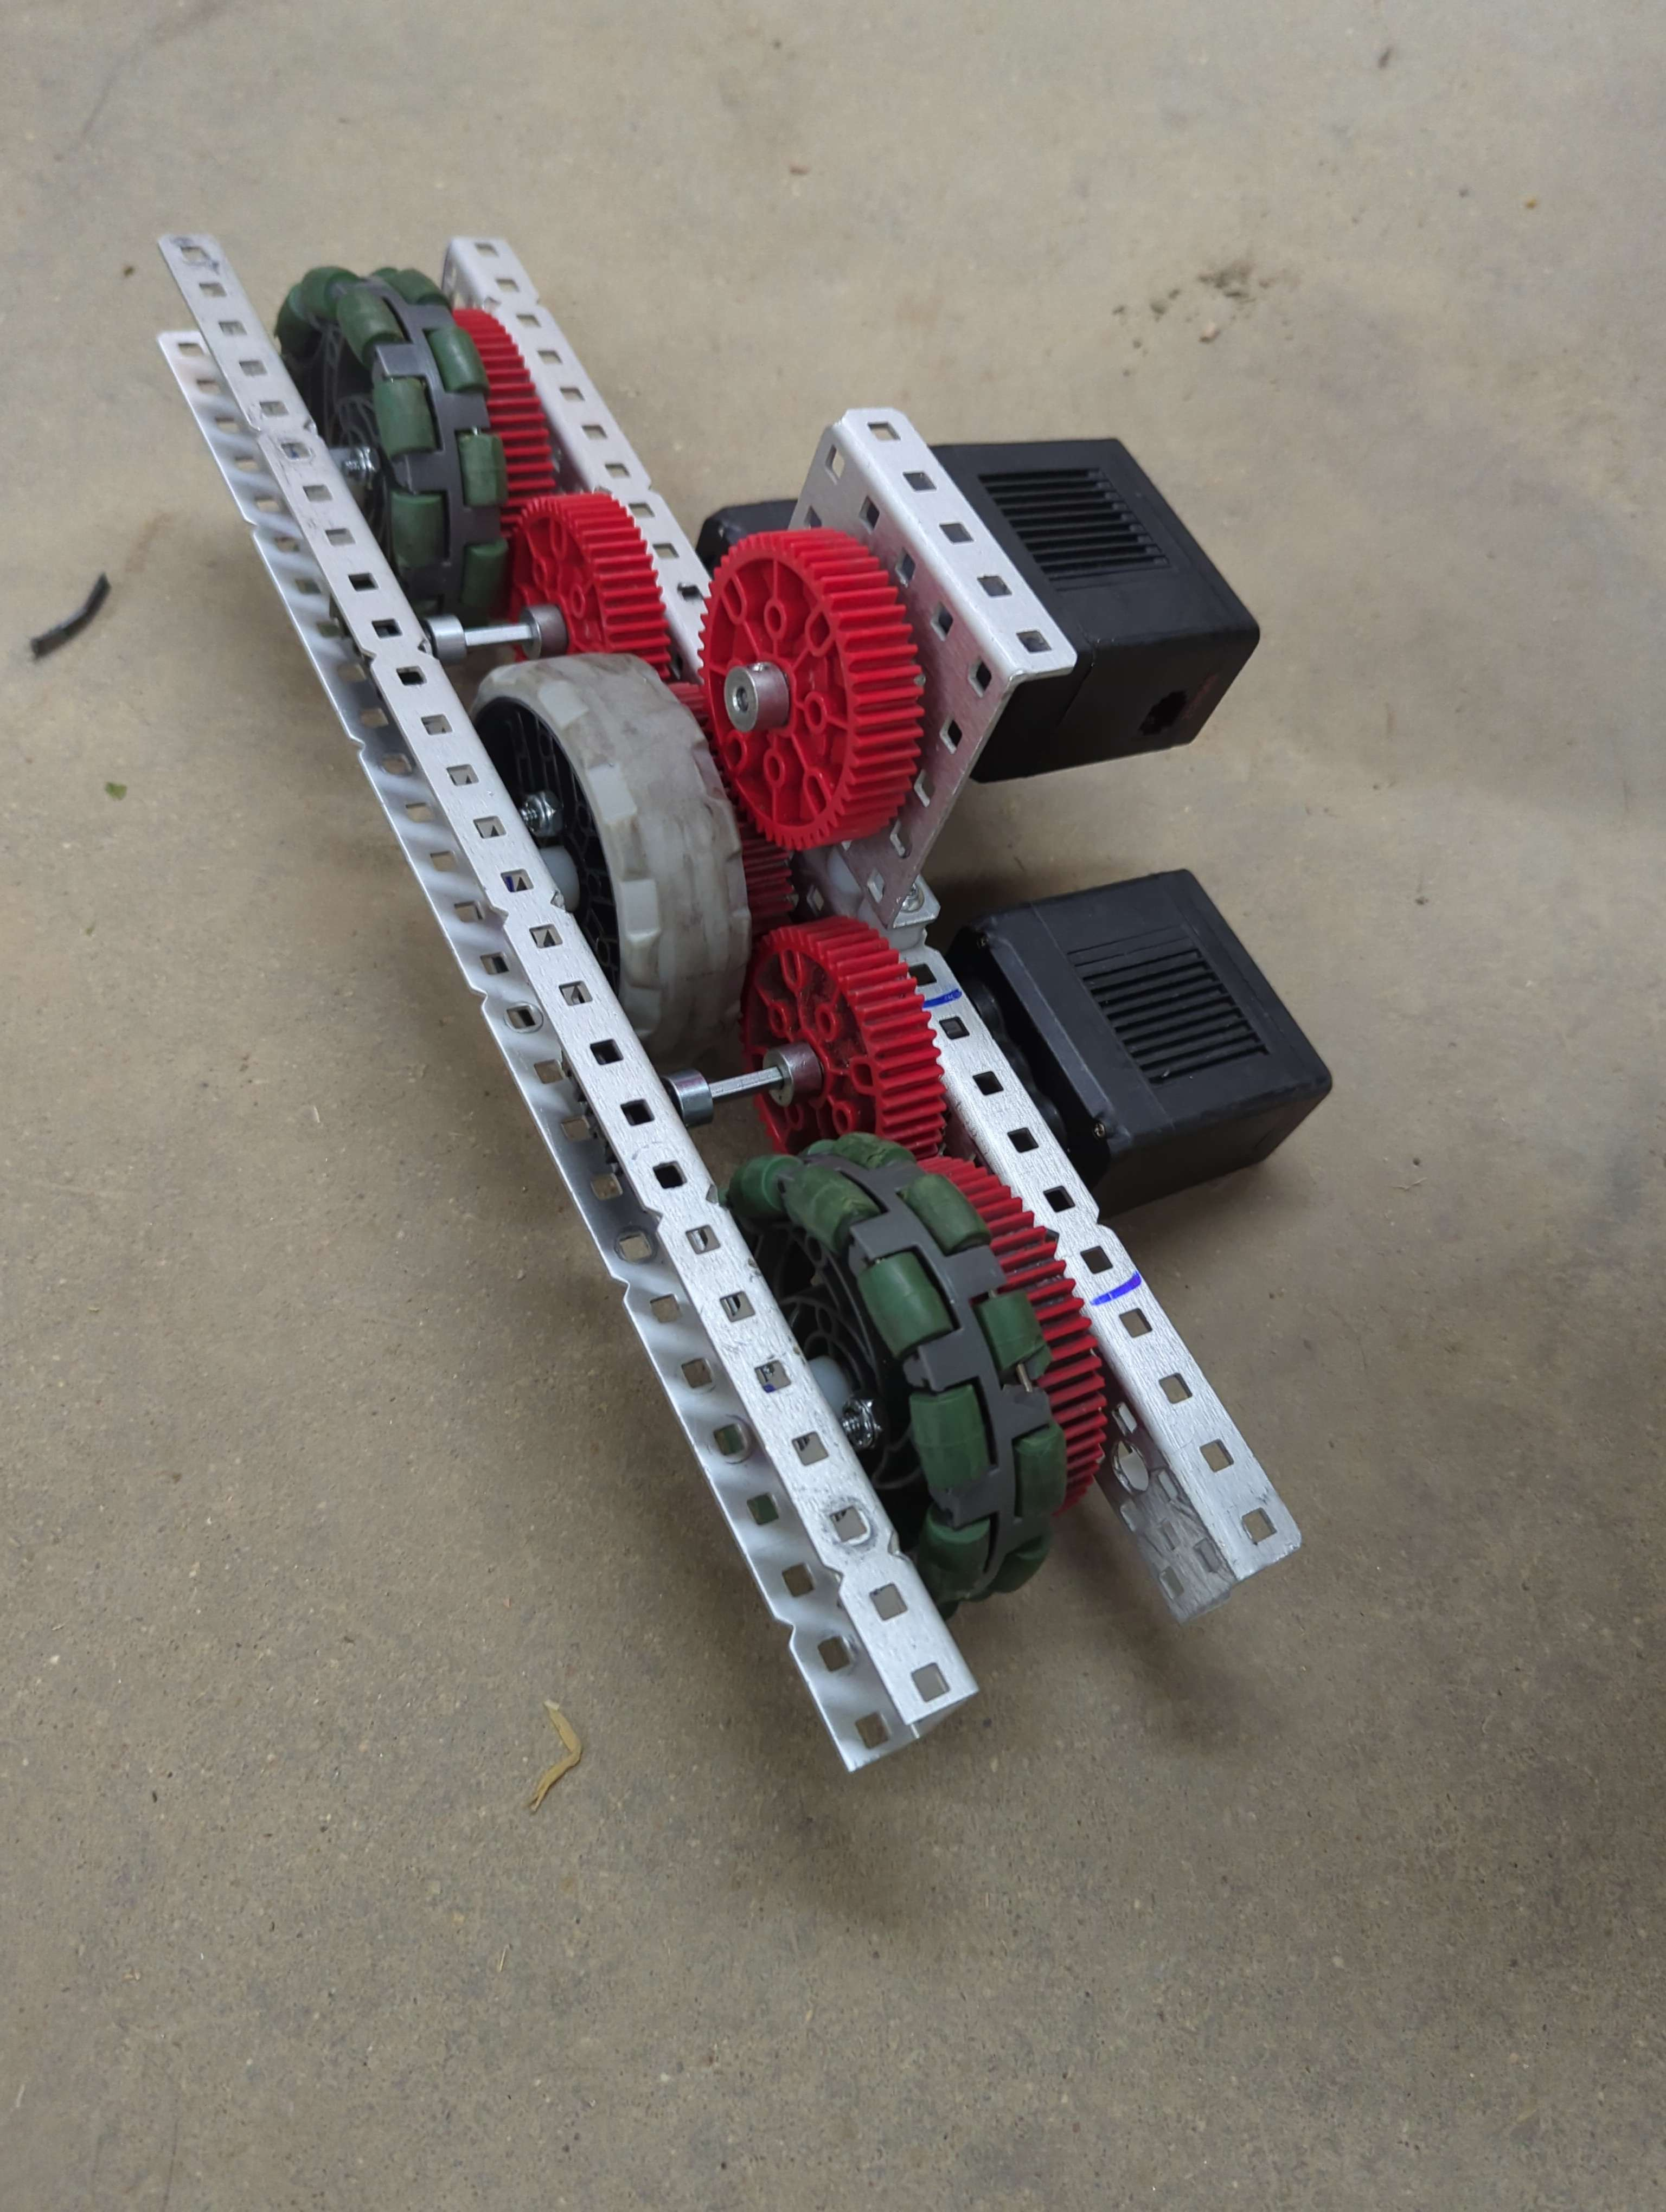
\includegraphics[width=.8\linewidth]{images/Full Drive.jpg}
        \caption{Single Side of Drive}
        \label{fig:side-of-drive}
    \end{minipage}
     \begin{minipage}{.5\textwidth}
        \centering
        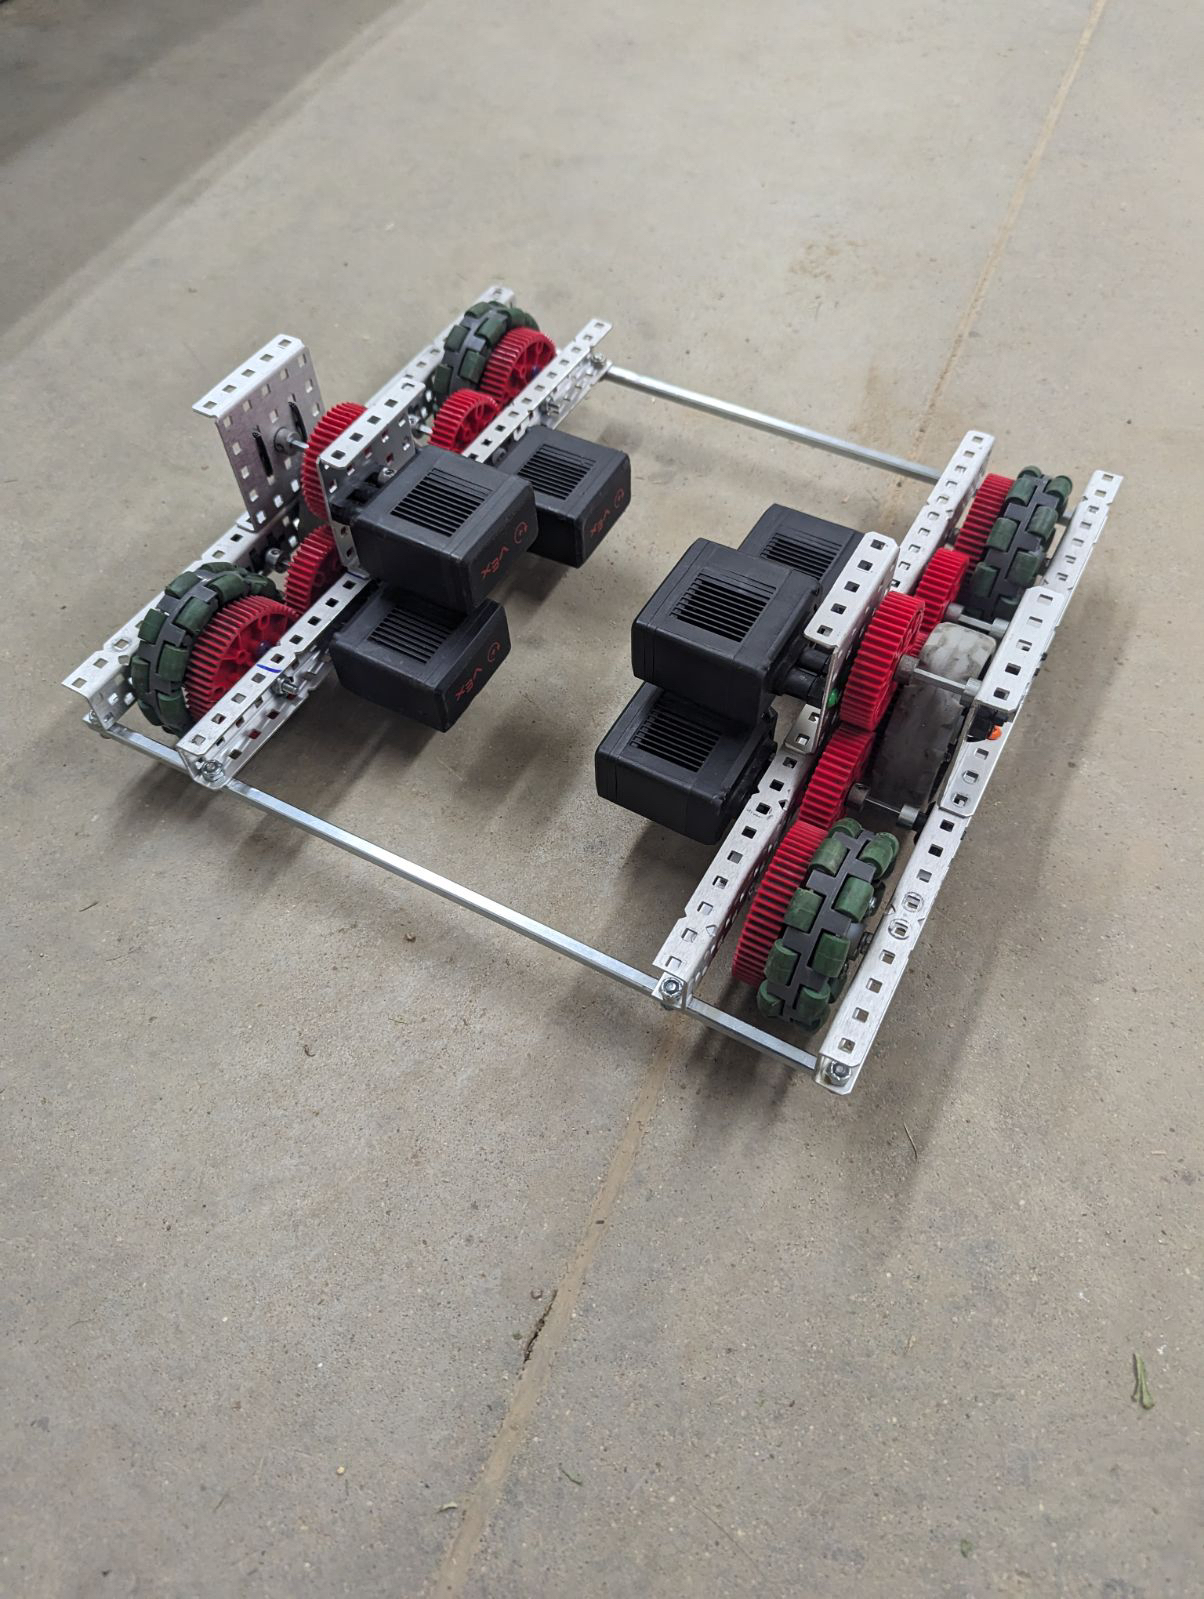
\includegraphics[width=.8\linewidth]{images/Drivetrain.jpg}
        \caption{Drivetrain}
        \label{fig:drivetrain}
    \end{minipage}
\end{figure}
\test{Test the Solution (June 8, 2024)}
\label{Test-the-Solution}
\chapterauthor{Caleb Bachmeier, Ian Smith}
\info{Caleb Bachmeier}{Test the Solution}{June 8, 2024}
\textbf{Goal}: Test our built drivetrain
    \section*{Test the Solution}
After temporarily mounting our brain, battery and radio to the robot, we coded it to drive using speed curves and curvature drive. Both of these are better explained in the next paragraph. By coding our drive in the same way it will be coded at competitions, we can let our drivers get a feel for the robot -- it is worth noting that this 'feel' with change as we add additional mechanisms to the robot. We still need to do some testing on our robot to ensure that our speed is correct, the equation to find our theoretical speed is:
\[
t = \frac{d}{v}
\]
Where
\begin{itemize}
    \item t is the time (in seconds),
    \item d is the distance (in inches), and
    \item v is the speed of the robot (in inches per second).
\end{itemize}
Using this data we will add in our expected result into the table below:

For 5 feet (60 inches):
\[
t = \frac{60}{82} \approx 0.73 \, \text{seconds}
\]

For 10 feet (120 inches):
\[
t = \frac{120}{82} \approx 1.46 \, \text{seconds}
\]

For 20 feet (240 inches):
\[
t = \frac{240}{82} \approx 2.93 \, \text{seconds}
\]

The formula for percent error is:

\[
\text{Percent Error} = \left( \frac{|\text{Experimental Value} - \text{Theoretical Value}|}{\text{Theoretical Value}} \right) \times 100
\]

\textbf{Variables}
\begin{itemize}
    \item Independent: length
    \item Dependant: time
    \item Constant Factors: 
    \begin{itemize}
        \item Same robot
        \item Floor were are testing on (The foam tiles on the VEX VRC field)
        \item Stopwatch
        \item Environment (Inside)
    \end{itemize}
\end{itemize}


\renewcommand{\arraystretch}{1.85} % Change this value as needed
\begin{table}[htb!]
\centering
\begin{tabular}{|>{\centering\arraybackslash}m{1.85cm}|>{\centering\arraybackslash}m{1.85cm}|>{\centering\arraybackslash}m{1.85cm}|>{\centering\arraybackslash}m{1.85cm}|>{\centering\arraybackslash}m{1.85cm}|>{\centering\arraybackslash}m{1.85cm}|>{\centering\arraybackslash}m{1.85cm}|}
\hline
\textbf{} & \textbf{5 Feet} & \textbf{10 Feet} & \textbf{20 Feet}
\tabularnewline
\hline
Expected Result & 0.73 seconds & 1.46 seconds & 2.93 seconds \tabularnewline
\hline
Actual Result & 0.84 seconds & 1.65 seconds & 2.95 seconds \tabularnewline
\hline
Difference & 0.11 seconds & 0.19 seconds & 0.02 seconds \tabularnewline
\hline
Percent Error & 15.07\% & 13.02\% &  0.68\% \tabularnewline
\hline
\end{tabular}
\caption{Drive Testing}
\end{table}
\renewcommand{\arraystretch}{1.85} % Reset to default
\pagebreak
\section*{Speed Curves and LemLib}

Below is a paragraph written by \blueref{Ian}{Ian Smith} on the Advantages of Speed and Steer Curves when driving:

\vspace{1cm}

The concept of a speed curve is used when discussing driver assists. At the most fundamental level, speed curves are used to allow the driver to have more precise control at lower joystick positions while sacrificing control at higher motor velocities. The reason this is advantageous is because a lower motor velocity is synonymous with requirements of finer driver control. Thus, more space on the joystick is given for areas at lower velocity where the drive may want to be more precise. This takes just a little bit of the fine motor control skill away from the driver itself and compensates mathematically. Originally when writing my first motor curve function, I originally used a switch.case argument using only linear functions. The next adaptation was an exponential curve using the base \(e\). However, the latest adaptation of motor curves was after using the LemLib library, where the motor curve functions were already built into the drivetrain class, saving me time having to modify some code. This forum has been a help in the later implementation of motor curves in combination with LemLib due to the nature of the way constants are layed out 

\href{https://www.vexforum.com/t/expo-drive-lemlibs-implementation/123337}{This is a link to VEX Forums about LemLib's Implementation into VRC}. \href{https://www.desmos.com/calculator/umicbymbnl}{Here is the interactive Desmos page developed by the LemLib team.}
